\chapter{Optimizing Nonrecursive Queries}
\label{chapter:spores}


Consider the Linear Algebra (LA) expression $sum((X-UV^T)^2)$ which
defines a typical loss function for approximating a matrix $X$ with a
low-rank matrix $UV^T$. Here, $sum()$ computes the sum of all matrix
entries in its argument, and $A^2$ squares the matrix $A$
element-wise. Suppose $X$ is a sparse, 1M x 500k matrix, and suppose
$U$ and $V$ are dense vectors of dimensions 1M and 500k respectively.
Thus, $UV^T$ is a rank 1 matrix of size 1M x 500k, and computing it
naively requires 0.5 trillion multiplications, plus memory allocation.
Fortunately, the expression is equivalent to
$sum(X^2) - 2U^TXV + U^TU * V^TV$.  Here $U^TXV$ is a scalar that can
be computed efficiently by taking advantage of the sparsity of $X$,
and, similarly, $U^TU$ and $V^TV$ are scalar values requiring only 1M
and 500k multiplications respectively.

Optimization opportunities like this are ubiquitous in machine
learning programs. State-of-the-art optimizing compilers such as
SystemML~\cite{DBLP:reference/bdt/Boehm19},
OptiML\cite{DBLP:conf/icml/SujeethLBRCWAOO11}, and
Cumulon\cite{DBLP:conf/sigmod/HuangB013} commonly implement syntactic
rewrite rules that exploit the algebraic properties of the LA
expressions. For example, SystemML includes a rule that rewrites the
preceding example to a specialized operator\footnote{See the
  \href{https://systemml.apache.org/docs/0.12.0/engine-dev-guide.html}{SystemML
    Engine Developer Guide} for details on the weighted-square loss
  operator \texttt{wsloss}. } to compute the result in a streaming
fashion.  However, such syntactic rules fail on the simplest
variations, for example SystemML fails to optimize $sum((X+UV^T)^2)$,
where we just replaced $-$ with $+$.  Moreover, rules may interact
with each other in complex ways.  In addition, complex ML programs
often have many common subexpressions (CSE), that further interact
with syntactic rules, for example the same expression $UV^T$ may occur
in multiple contexts, each requiring different optimization rules.

In this chapter we describe \sys, a novel optimization approach for
complex linear algebra programs that leverages relational algebra as
an intermediate representation to completely represent the search
space. SPORES first transforms LA expressions into traditional
Relational Algebra (RA) expressions consisting of joins, unions 
and aggregates.  It then performs a cost-based optimizations on
the resulting Relational Algebra expressions, using only standard
identities in RA.  Finally, the resulting RA expression is converted
back to LA, and executed.

A major advantage of \sys\ is that the rewrite rules in RA are
complete.  Linear Algebra seems to require an endless supply of clever
rewrite rules, but, in contrast, by converting to RA, we can prove
that our set of just 13 rules are complete. The RA expressions in this dissertation are
over $K$-relations~\cite{DBLP:conf/pods/GreenKT07}; a tuple $X(i,j)$
is no longer true or false, but has a numerical value, e.g. $5$,
%
which could be interpreted, e.g., as the multiplicity of that tuple.
%
In other words, the RA expressions that result from LA expressions are
interpreted over bags instead of sets. 
\rvo{The problem of checking equivalence of
queries under bag semantics has a unique history.  Chaudhuri and Vardi
first studied the containment and equivalence problem under bag
semantics, and claimed that two conjunctive queries are equivalent iff
they are isomorphic: Theorem 5.2
in~\cite{DBLP:conf/pods/ChaudhuriV93}.  However, a proof was never
produced.  A rather long proof for this claim was given for the
bag-set semantics in~\cite{DBLP:journals/tocl/CohenSN05}.  Green
provided a comprehensive proof, showing that two unions of conjunctive
queries (UCQ) are equivalent under bag semantics iff they are
isomorphic, by using sophisticated techniques involving multiple
semirings~\cite{DBLP:conf/icdt/Green09}.  The completeness result of
our 13 rules relies on a similar result, but stated for tensors rather
than bags; we present here a simple and self-contained proof in
Sec.~\ref{ranf}.  We note that, in contrast, {\em containment} of two
UCQs with bag semantics is
undecidable~\cite{DBLP:journals/tods/IoannidisR95}; we do not consider
containment in this dissertation.
}
Finally, we prove that our optimizer rules are
sufficient to convert any RA expression into its {\em canonical form},
i.e.  to an UCQ, and thus can, in principle, discover all equivalent
rewritings.

However, we faced a major challenge in trying to exploit the
completeness of the rules.  The search space is very large,
typically larger than that encountered in standard database
optimizers, because of the prevalence of unions $+$, large number of
aggregates $\sum$, and frequent common subexpressions. To tackle this,
\sys\ adopts and extends a technique from compilers called {\em
  equality saturation}~\cite{DBLP:journals/corr/abs-1012-1802}.
It uses a data structure called the E-Graph \cite{10.5555/909447} to
compactly represent the space of equivalent expressions, and equality
rules to populate the E-Graph, then leverages constraint solvers to
extract the optimal expression from the E-Graph. \rvo{We extend equality
saturation with rule sampling and use a greedy extraction algorithm
to quickly cover vast portions of the search space, and trade the
guarantee of optimality for shorter compile time.} 

We have integrated \sys\ into
SystemML~\cite{DBLP:reference/bdt/Boehm19}, and show that it can
derive all hand-coded rules of SystemML.  We evaluated \sys\ on a
spectrum of machine learning tasks, showing competitive performance
improvement compared with more mature heuristic-based optimizers. Our
optimizer rediscovers all optimizations by the latter, and also finds
new optimizations that contribute to \rvo{up to 10X speedup}.

We make the following contributions in this dissertation:
\begin{enumerate}
\item We describe a novel approach for optimizing complex Linear
  Algebra expressions by converting them to Relational Algebra, \rvo{and
  prove the completeness of our rewrite rules} (Sec.~\ref{sec:la:to:ra}).
\item We present a search algorithm based on Equality Saturation that
  can explore a large search space while reusing memory (Sec.~\ref{explore}).
\item We conduct an empirical evaluation of the optimizer using
  several real-world machine learning tasks, and demonstrate it's
  superiority over an heuristics-driven optimizer in SystemML
  (Sec.~\ref{sec:evaluation}).
\end{enumerate}{}

\section{Representing the Search Space} \label{sec:la:to:ra}

\subsection{Rules \texorpdfstring{$R_{LR}$}{R\_LR}: from  LA to RA and Back}
In this section we describe our approach of optimizing LA expressions
by converting them to RA.  The rules converting from LA to RA and back
are denoted $R_{LR}$.

To justify our approach, let us revisit our example loss function
written in LA and attempt to optimize it using standard LA identities.
Here we focus on algebraic rewrites and put aside concerns about the
cost model. Using the usual identities on linear algebra expressions,
one may attempt to rewrite the original expression as follows:
\begin{align*}
& sum((X-UV^T)^2) \\
= &sum((X-UV^T)*(X-UV^T)) \\
=&sum(X^2-2X*UV^T+(UV^T)^2) \\
= & sum(X^2) - 2sum(X*UV^T) + sum((UV^T)^2)
\end{align*}
% \dan{$(UV^T)^2$ should be $sum(UV^T)^2$.}
At this point we are stuck trying to rewrite $sum(X*UV^T)$ (recall
that $*$ is element-wise multiplication); it turns out to be equal to
$sum(U^TXV)$, for any matrices $X,U,V$ (and it is equal to the scalar
$U^TXV$ when $U, V$ are column vectors), but this does not seem to
follow from standard LA identities like associativity, commutativity,
and distributivity.  Similarly, we are stuck trying to rewrite
$sum((UV^T)^2)$ to $sum(U^TU * V^TV)$.  Current systems manually add
syntactic rewrite rules, whenever such a special case is deemed
frequent enough to justify extending the optimizer.


\begin{table}
\caption{Representation of expressions in LA and RA.}
\vspace{3pt}
\centering
%%% (Dan: I replaced the multiplicies 1,2 with different ones so
%%% readers don't confuse them with indices in the matrix)
\begin{tabular}{@{}ccccc@{}}
&
     $A$ & $x$ & $A * x^T$ & $Ax$\\
     \hline
     \\[-1em]
LA &
     $\begin{bmatrix}
    0 & 5 \\
    7 & 0
    \end{bmatrix}$ & $\begin{bmatrix}
    3\\
    2
    \end{bmatrix}$ & $\begin{bmatrix}
    0 & 10 \\
    21 & 0
    \end{bmatrix}$ & $\begin{bmatrix}
    10 \\
    21
    \end{bmatrix}$ \\
    \\[-0.8em]
    \hline
RA &
    \begin{tabular}{|c|c|c}
    $i$ &$j$&\# \\
    \hline
        $1$ & $2$ & 5 \\
        $2$ & $1$ & 7
    \end{tabular}{} &
    \begin{tabular}{|c|c}
         $j$ &\# \\
         \hline
         1 & 3\\
         2 & 2
    \end{tabular}{} &
    \begin{tabular}{|c|c|c}
    $i$ &$j$ & \# \\
    \hline
        $1$ & $2$ & 10 \\
        $2$ & $1$ & 21
    \end{tabular}{} &
    \begin{tabular}{|c|c}
         $i$ & \# \\
         \hline
         1 & 10 \\
         2 & 21
    \end{tabular}{} 
\end{tabular}{}
    % \caption{Top: Linear Algebra manipulates matrices and vectors.
%   $A*x^T$ is (broadcasting) element-wise multiplication, computing the matrix
%   $(A_{ij}x_j)_{ij}$, while $Ax$ is standard matrix-vector
%   multiplication.  Bottom: their translations into $K$-relations and
%   Relational Algebra operations.  Each relation is a bag, where the
%   attribute $\#$ represents the multiplicity, i.e. $A(1,2)$ has
%   multiplicity $5$ etc.  Then $A*x^T$ becomes a standard query
%   $Q(i,j) = A(i,j) \times x(j)$, while $Ax$ is a query with a group-by and
%   aggregate, $Q(i) = \sum_j A(i,j) \times x(j)$.}
    \label{matrixkrel}
    \vspace*{8pt}
\end{table}{}

Instead, our approach is to expand out the LA expression element-wise.
For example, assuming for simplicity that $U,V$ are column vectors, we
obtain
\begin{align*}
& sum((UV^T)^2) = \textstyle{\sum_{i,j}} (U_i \times V_j) \times (U_i \times V_j) \\
& = \textstyle{\sum_{i,j}}(U_i \times U_i) \times (V_j \times V_j) \\
& = ( \textstyle{\sum_i} U_i \times U_i) \times ( \textstyle{\sum_j} V_j \times V_j)  \\
& = U^TU \times V^TV
\end{align*}
%
The expressions using indices represent Relational Algebra
expressions.  More precisely, we interpret every vector, or matrix, or
tensor, as a $K$-relation~\cite{DBLP:conf/pods/GreenKT07} over the
reals. In other words we view $X_{ij}$ as a tuple $X(i,j)$ whose
``multiplicity'' is the real value of that matrix element.  We
interpret point-wise multiply as natural join; addition as union; sum
as aggregate; and matrix multiply as aggregate over a join\footnote{In
  the implementation, we use outer join for point-wise multiply and
  addition, where we multiply and add the matrix entries
  accordingly. In this chapter we use join and union to simplify
  presentation.}.
%
Table~\ref{matrixkrel} illustrates the correspondence between LA and
RA.  We treat each matrix entry $A_{ij}$ as the multiplicity of tuple
$(i, j)$ in relation $A$ under bag semantics. For example
$A_{2,1} = 7$, therefore the tuple $(2,1)$ has multiplicity of $7$ in
the corresponding relation. \rvt{The relation schema stores the size of each dimension.}
$A*x^T$ denotes element-wise
multiplication, where each element $A_{ij}$ of the matrix is
multiplied with the element $x_j$ of the row-vector $x^T$.  In RA it
is naturally interpreted as the natural join $A(i,j) \Join x(j)$,
which we write as $A(i,j) \times x(j)$.  Similarly, $Ax$ is the standard
matrix-vector multiplication in LA, while in RA it becomes a query
with a group by and aggregate, which we write as $\sum_j A(i,j) \times x(j)$.
Our $K$-relations are more general than bags, since the entry of a
matrix can be a real number, or a negative number; they correspond to
$K$-relations over the semiring of reals $(\R, 0, 1, +, \times)$.

% Of course, a matrix can have an entry that is not an integer, which
% would not make sense as multiplicity. In general, the matrix entries
% corresponds to the semiring of reals which serve as relation
% annotations \cite{DBLP:conf/pods/GreenKT07} in the $K$-relation.
\begin{table}
\caption{LA and RA operators. The type $M_{M,N}$ is a matrix of size $M \times
  N$; $[i,j]$ is a list of attribute names; $R_{i:M,j:N}$ is a relation with
  attributes $i$ of size $M$ and $j$ of size $N$; $S_1, S_2, S,$ and $U$ are
  sets of attributes. \rvt{\texttt{elemmult} and \texttt{elemplus} are broadcasting.}}
\begin{tabular}{llll}
&name & type & syntax \\ \hline \multirow{7}{*}{\rotatebox[origin=c]{90}{LA}}
  &mmult & $M_{M,L} \times M_{L,N} \rightarrow M_{M,N}$ & $AB$ 
  \\ &elemmult & $M_{M,N} \times M_{M,N} \rightarrow M_{M,N}$ & $A*B$
  \\ &elemplus & $M_{M,N} \times M_{M,N} \rightarrow M_{M,N}$ & $A+B$ \\ &rowagg
  & $M_{M,N} \rightarrow M_{M,1}$ & $sum_{row} A$ \\ &colagg & $M_{M,N}
  \rightarrow M_{1,N}$ & $sum_{col} A$ \\ &agg & $M_{M,N} \rightarrow M_{1,1}$ &
  $sum A$ \\
%&power & $M  \times Int \rightarrow M$ & $A^k$ \\
&transpose & $M_{M,N} \rightarrow M_{N,M}$ & $A^\tr$ \\ \hline
  \multirow{2}{*}{\rotatebox[origin=c]{90}{conv.}} &bind & $M_{M,N} \times [i,j]
  \rightarrow R_{i:M,j:N}$ & $\bind{i,j} A$ \\ &unbind & $R_{i:M,j:N} \times
              [i,j] \rightarrow M_{M,N}$ & $\unbind{i}{j} A$ \\ \hline
              \multirow{2}{*}{\rotatebox[origin=c]{90}{RA}} &join & $R_{S_1}
              \times R_{S_2} \rightarrow R_{S_1 \cup S_2}$ & $A \rmul B$
              \\ &union & $R_{S_1} \times R_{S_2} \rightarrow R_{S_1 \cup S_2}$
              & $A \radd B$ \\ &agg & $R_S \times U \rightarrow R_{S \setminus
                U}$ & $\sum_{U} A$ \\
\end{tabular}

\label{tPlanOps}
\end{table}
\begin{figure}
\begin{enumerate}
\itemsep0em
  \item $A*B \rightarrow \unbind{i}{j}(\bind{i,j}A \rmul \bind{i,j}B)$.
  \item $A+B \rightarrow \unbind{i}{j}(\bind{i,j}A \radd \bind{i,j}B)$.
  \item $sum_{row} A \rightarrow [-i,\_ ] \sum_j \bind{i,j} A$. Similar for
    $sum_{col}$, $sum$.
  \item $AB \rightarrow \unbind{i}{k} \sum_j (\bind{i,j}A \rmul \bind{j,k}B)$.
  \item $A^\tr \rightarrow \unbind{j}{i} \bind{i,j}A$.
  \item $A - B \rightarrow A + (-1) * B$
\end{enumerate}
\caption{LA-to-RA Ruleset $R_{LR}$.}
\vspace*{3pt}
\label{RMR}
\end{figure}

% Following our relational semantics, $sum((X-UV^T)^2)$ is interpreted
% as
% $\sum_{ij} (X_{ij} - U_{i} \bowtie V_{j}) \bowtie (X_{ij} - U_{i}
% \bowtie V_{j})$. Note that because $U$ and $V$ are vectors, the
% aggregate in their matrix product $\sum_{\varnothing} U_i \bowtie V_j$
% is over an empty set of attributes and therefore eliminated.
% Hereafter we will overload $*$ for join and $+$ for union to keep our
% formulas intuitive.  Table~\ref{tPlanOps} provides the list of LA and
% RA operators.  

We now describe the general approach in \sys.  The definition
of LA and RA are in Table~\ref{tPlanOps}.  LA consists of seven
operators, which are those supported in
SystemML~\cite{DBLP:reference/bdt/Boehm19}. \rvt{These operators all 
implement sum-product operations and take up the majority of run
time in machine learning programs as we show in Section~\ref{perf}.
We also support common operations like division and logarithm as we
discuss in Section~\ref{udfs}.} RA consists of only three
operators: $\times$ (natural join), $+$ (union), and $\sum$ (group-by
aggregate).  Difference is represented as $A-B = A + (-1)B$ (this is
difference in $\R$; we do not support bag difference, i.e.  difference
in $\N$ like $3-5=0$, because there is no corresponding operation in
LA), while selection can be encoded by multiplication with relations
with 0/1 entries.  We call an expression using these three RA
operators an {\em RPlan}, for Relational Plan, and use the terms RPlan
and RA/relational algebra interchangeably.  Finally, there are two
operators, {\em bind} and {\em unbind} for converting between
matrices/vectors and $K$-relations.


The translation from LA to RA is achieved by a set of rules, denoted
$R_{LR}$, and shown in Figure~\ref{RMR}. The bind operator
$\bind{i,j}$ converts a matrix to a relation by giving attributes
$i,j$ to its two dimensions; the unbind operator $\unbind{i}{j}$
converts a relation back to a matrix. For example,
$\unbind{j}{i}\bind{i,j}A$ binds $A$'s row indices to $i$ and its
column indices to $j$, then unbinds them in the opposite order,
thereby transposing $A$.

\sys\ translates a complex LA expression into RA by first applying the
rules $R_{LR}$ in Figure~\ref{RMR} to each LA operator, replacing it
with an RA operator, preceded by {\em bind} and followed by {\em
  unbind}. Next, it eliminates consecutive unbind/bind operators,
possibly renaming attributes, e.g.  $\bind{k,l} \unbind{i}{j} A$
becomes $A[i \to k, j \to l]$, which indicates that the attributes $i$
and $j$ in $A$'s schema should be renamed to $k$ and $l$, by
propagating the rename downward into $A$.  As a result, the entire LA
expression becomes an RA expression (RPlan), with {\em bind}
on the leaves and {\em unbind} at the top.

\begin{figure}
\begin{enumerate}
\itemsep0em
  \item\label{RRC_mp} $A \rmul (B \radd C) = A \rmul B \radd A \rmul C$
  \item\label{RRC_ap} $\sum_i (A \radd B) = \sum_i A \radd \sum_i B$
  \item\label{RRC_ma} If $i \not\in A$, $A \rmul \sum_i B = \sum_i (A \rmul B)
    \quad$ (else rename $i$)
  \item\label{RRC_aa} $\sum_i \sum_j A = \sum_{i,j} A$
%   \item $\sum_i A \rightarrow \sum_{i,j} A$
  \item\label{RRC_ac} If $i \not\in Attr(A)$, then $\sum_i A = A \rmul dim(i)$
  \item\label{RRC_pp} $A \radd (B \radd C) = +(A, B, C) \quad$ (assoc. \& comm.)
  \item\label{RRC_mm} $A \rmul (B \rmul C) = \times (A, B, C) \quad$ (assoc. \& comm.)
\end{enumerate}
\caption{RA equality rules $R_{EQ}$.}
\label{RRC}
\vspace*{3pt}
\end{figure}


% \begin{figure}
%     \centering
%     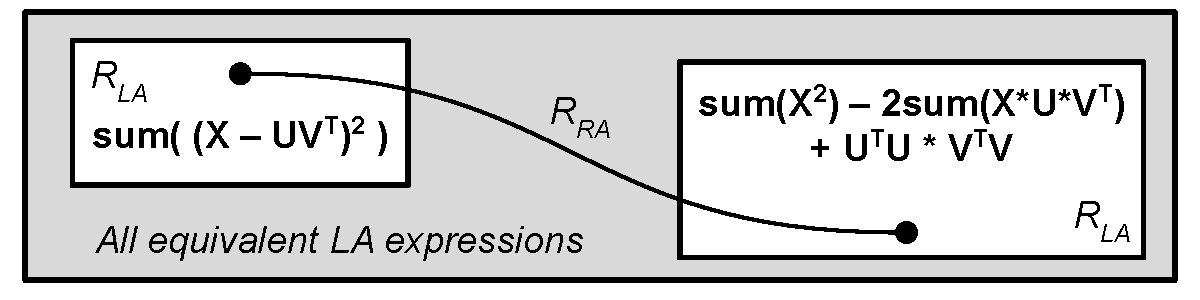
\includegraphics[width=0.8\linewidth]{wormhole}
%     \caption{Venn diagram of LA and/or RA expressions.}
%     \label{wormhole}
% \end{figure}{}

% \begin{figure}
%     \centering
% \begin{tikzcd}
% e_{LA} \arrow[rr, "=" description, no head, dotted] \arrow[d, "R_{LR}"'] &           & e'_{LA} \arrow[d, "R_{LR}"]  \\
% e_{RA} \arrow[r, "R_{EQ}"]                                               & \mathcal{C}(e_{RA}) \equiv \mathcal{C}(e'_{RA})  & e'_{RA} \arrow[l, "R_{EQ}"']
% \end{tikzcd}
    
%     \caption{Two LA expressions $e_{LA}$ and $e'_{LA}$ are equivalent \textit{iff} their
%     relational counterparts $e_{RA}$ and $e'_{RA}$ have isomorphic
%       canonical forms $\mathcal{C}(e_{RA}), \mathcal{C}(e'_{RA})$. $R_{LR}$ translates a LA expression to RA and $R_{EQ}$ are the relational equality rules. }
%     \label{proofsketch}
% \end{figure}{}

% \begin{figure}
%     \centering
%     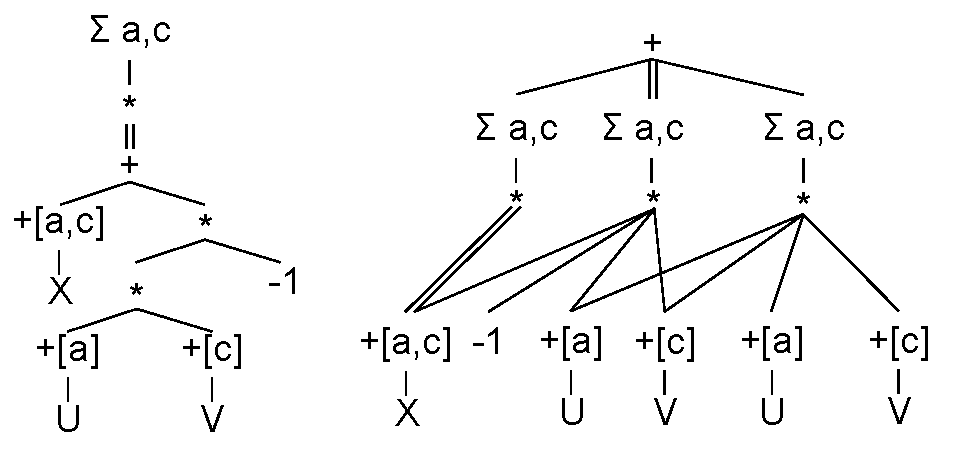
\includegraphics[width=0.9\linewidth]{img/radags.pdf}
%     \caption{RA DAGs for $sum((X-UV^T)^2)$ (left) and its canonical form (right). 
%     % \label{fig:radags}
% \end{figure}{}

% \begin{figure*}
%     \centering 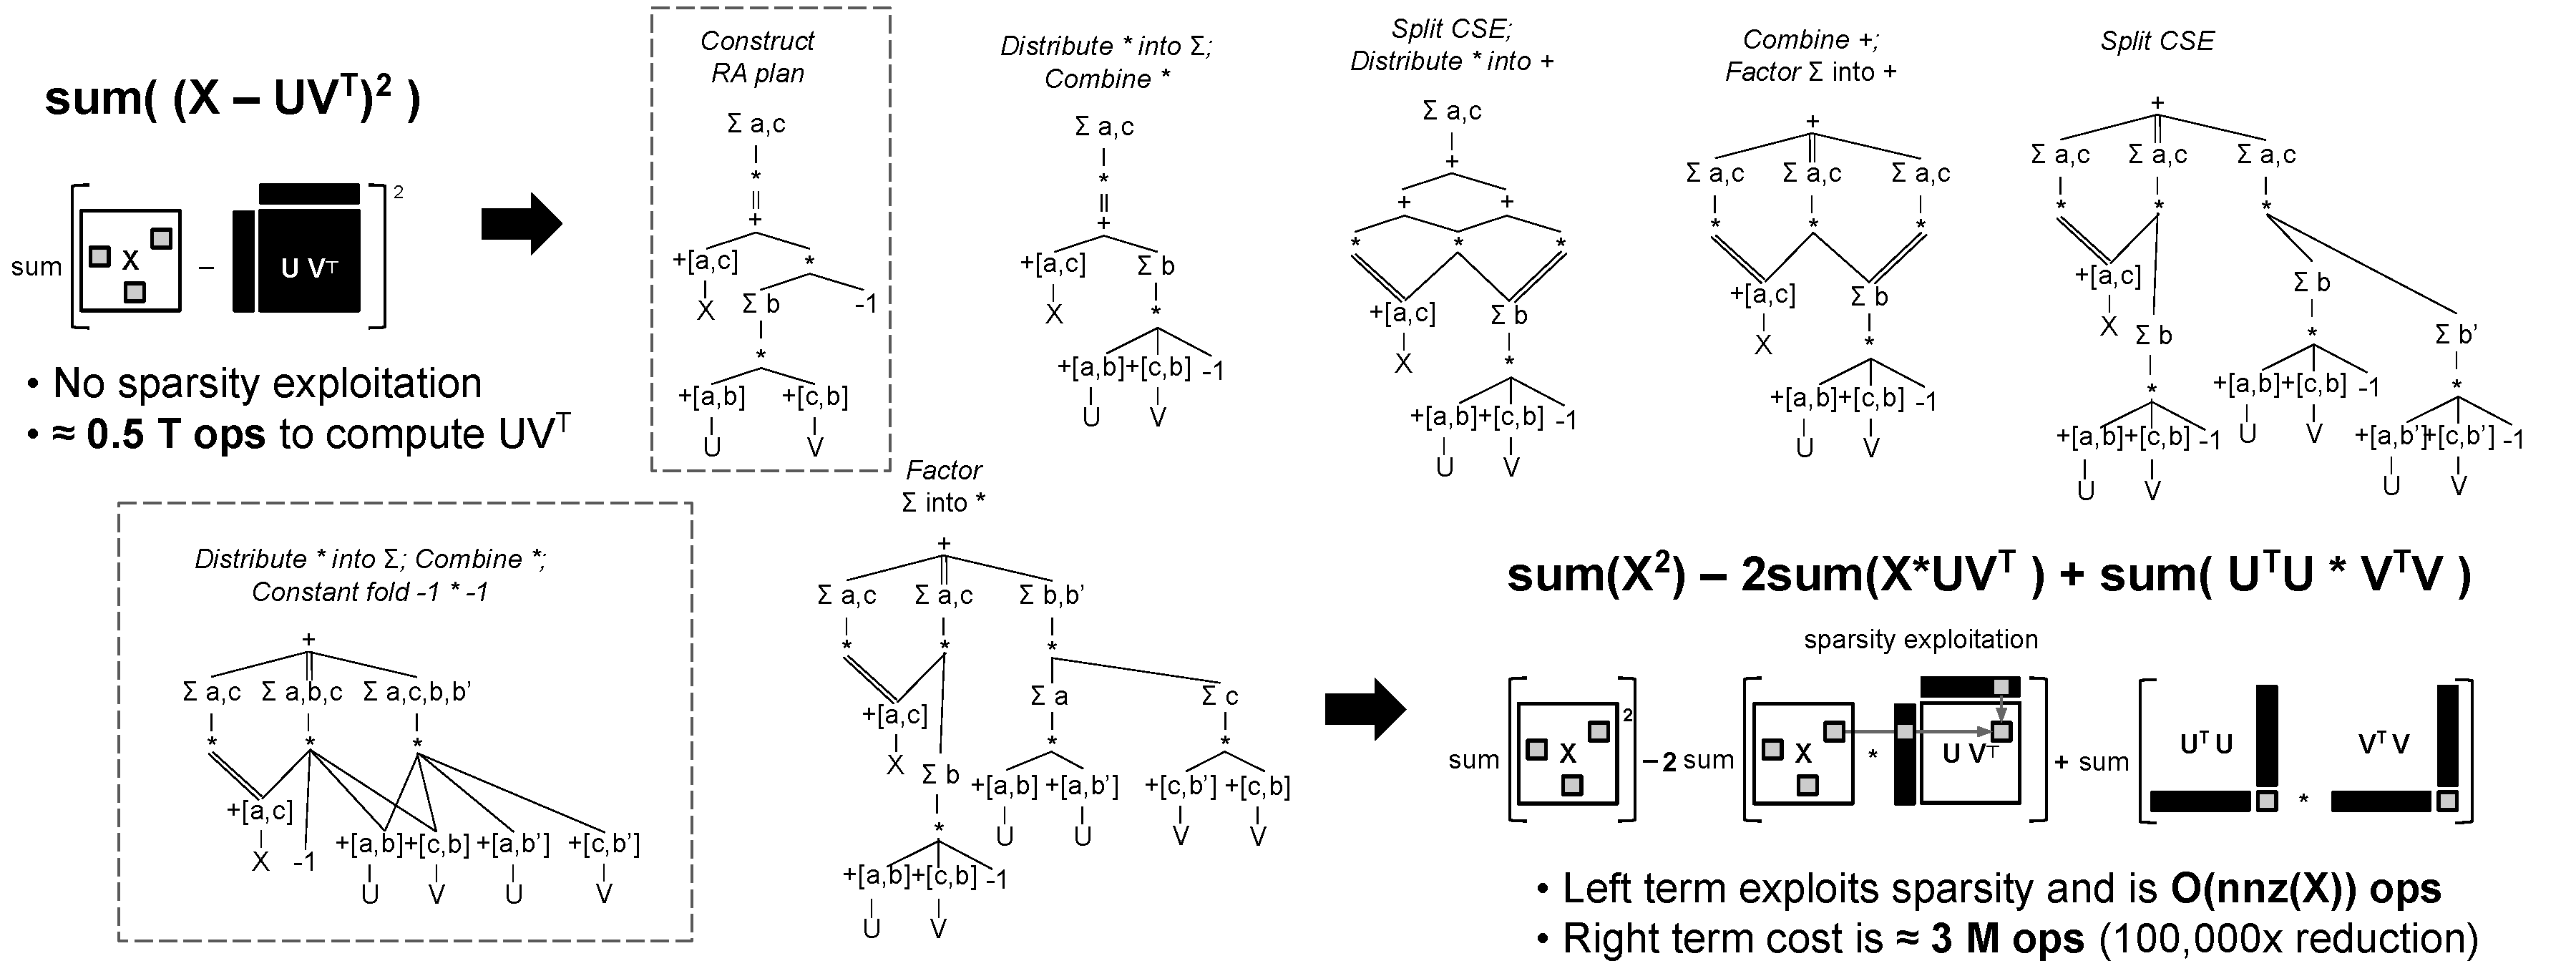
\includegraphics[width=\textwidth]{parrot}
%     \caption{Rewriting details using $R_{LR}$ and $R_{EQ}$ and the
%       optimization's impact on execution cost. Here we show the general case
%       where $U$ and $V$ are matrices, and $X*UV^T$ is computed with a fused
%       chain multiplication operator that exploits sparsity. Dashed lines
%       highlight the initial RPlan and its canonical form. }
%     \label{parrot}
% \end{figure*}




\subsection{Rules \texorpdfstring{$R_{EQ}$}{R\_EQ} : from RA to RA}

The equational rules for RA consists of seven identities shown in
Figure~\ref{RRC}, and denoted by $R_{EQ}$.  The seven rules are
natural relational algebra identities, where $\times$ corresponds to
natural join, $+$ to union (of relations with the same schema) and
$\sum_i$ to group-by and aggregate.  In rule~\ref{RRC_ac},
$i \notin Attr(A)$ means that $i$ is not an attribute of $A$, and
$dim(i)$ is the dimension of index $i$.  For a very simple
illustration of this rule, consider $\sum_i 5$.  Here $5$ is a
constant, i.e. a relation of zero arity, with no attributes.  The rule
rewrites it to $5 dim(i)$, where $dim(i)$ is a number representing the
dimension of $i$.

%%% (Dan: I think the example below is wrong. In RA you must have
%%% indices, can't write $x+1$.
%  $\sum_i (x + 1)$ where $x$ is a vector of length 10 and
% $x + 1$ adds $1$ with each entry of $x$. Following rule~\ref{RRC_ap},
% pushing down the summation rewrites the expression to
% $\sum_i x + \sum_i 1$, and now rule~\ref{RRC_ac} rewrites $\sum_i 1$
% to $|i| * 1 = 10$.


\subsection{\rvo{Completeness of the Optimization Rules}}\label{ranf}

As we have seen at the beginning of this section, when rewriting LA
expressions using identities in linear algebra we may get stuck. Instead, by
rewriting the expressions to RA, the seven identities in $R_{EQ}$ are
much more powerful, and can discover more rewrites.
We prove
here that this approach is {\em complete}, meaning that, if two LA
expressions are semantically equivalent, then their equivalence can be
proven by using rules $R_{EQ}$.  The proof consists of two parts: (1)
the rules $R_{EQ}$ are sufficient to convert any RA expression $e$ to
its {\em normal form} (also called {\em canonical form})
$\mathcal{C}(e)$, and back, (2) two RA expressions $e, e'$ are
semantically equivalent iff they have isomorphic normal forms,
$\mathcal{C}(e) \equiv \mathcal{C}(e')$.
% 
% 
% 
% In general, any equivalent LA expressions can be rewritten to each other using
% our RA representation and equalities. In other words, the relational equalities
% $R_{EQ}$ are \textit{complete} w.r.t. linear algebra semantics. For
% optimization, this means RPlan and its equalities completely represent the
% search space of the optimization problem: we can rewrite an LA expression to any
% of its equals if we first translate it into RA, then apply a chain of equalities
% from $R_{EQ}$, and finally translate the result back to LA. As
% Figure~\ref{wormhole} illustrates, while the usual linear algebra identities
% $R_{LA}$ can only create disjoint equality space for our example expression pre-
% and post-optimization, the relational rules connects the space and rewrite the
% slow expression to the fast one. We sketch a proof of completeness in this
% section.
% 
% Figure~\ref{proofsketch} shows the main steps at a high level: two LA
% expressions are semantically equivalent if and only if their canonical
% form in RA are isomorphic, where $R_{LR}$ translates each expression
% to RA and $R_{EQ}$ takes the RA expression to its canonical form.

% Throughout this section we write $e\ R_{EQ}^*\ e'$ when $e, e'$ can be
% proven equal by using the identities in $R_{EQ}$ (Fig.~\ref{RRC}).

% By semantically equivalent, we
% mean two expressions evaluate to the same result given any same input (variable
% assignment). We define isomorphism of RA canonical forms in Section~\ref{ranf}.
We first give formal definitions for several important constructs. First, we interpret a relation as a function from {\em tuples} to a {\em semiring}. For simplicity we assume all attributes have the same domain $\D$. 
\begin{defn}{{\em (Relations)}}
  Fix a semiring $\SR$.  An {\em $\SR$-\textbf{relation}} is a function $A: \D^a \rightarrow \SR$ where $a$ is the {\em arity} of the relation.
% We write $|\D|$ for the size of domain $\D$. 
\end{defn}
When $\SR=\N$, then an $\N$-relation is a standard relation under bag semantics. When the domain is $\D = [n]$ for some natural number $n$ and $\SR=\R$, then an $\R$-relation is a tensor over the reals.  Next we define expressions over operators from Table~\ref{tPlanOps}. 

\begin{defn}{{\em (Expressions)}}\label{raexpr}
An expression in RA is either \begin{enumerate*}
    \item an \emph{\textbf{atom}} $r$ of the form $R(x_1, ..., x_a)$ where $R$ is a relation name and $(x_1, ..., x_a)$ a tuple of variables and/or constants, or
    \item a {\em natural join} of two expressions $e_1 \times e_2$, or 
    \item a {\em  union} of two expressions, $e_1 + e_2$, or
    \item an {\em aggregate},  $\sum_x e$. 
\end{enumerate*}{}
\end{defn}{}
Because the order of consecutive aggregates does not matter, we write $\sum_{\set{x_1, \dots, x_n}} e$ for $\sum_{x_1} \dots \sum_{x_n} e$. 
Given an expression $e$, we say that a variable $x$ is \emph{\textbf{bound}} in $e$, if $e$ contains an aggregate of the form $\sum_x e'$; 
otherwise it is \emph{\textbf{free}}. We write $vars(e)$ for the set of variables in $e$, $bv(t)$ for the set of bound variables, and $fv(t)$ for the set of free variables.
We interpret every expression $e$ as a lambda expression $\lambda fv(e) . e$ where the parameters $fv(e)$ may follow a given order, e.g. from an unbind operator if $e$ was converted from LA\footnote{A bind operator $[i,j]$ converts a matrix $A$ to an atom $A(i,j)$.}.
 In the body of the lambda expression, any atom $R(x_1, \dots , x_a)$ evaluates to some $s \in \SR$, and $+, \times$ and $\sum$ compute over $\SR$. We say two RA expressions are equivalent iff they evaluate to the same result given any same inputs: 

\begin{defn}{\em (Equivalence of Expressions)} Fix  expressions $e_1, e_2$ over the relation symbols $R_1, \ldots, R_n$.  We say that $e_1, e_2$ are {\em \textbf{equivalent}} over the semiring $\SR$ and the domain $\D$ if they have the same free variables, and for all interpretations $\pmb{I} = (R_1^I, \ldots, R_n^I)$ where $R_j^I : \D^{a_j} \rightarrow \SR$ for $j=1, \ldots, n$ the two expressions return the same answer, $e_1(\pmb{I}) = e_2(\pmb{I})$.  We write $e_1 =_{\SR, \D} e_2$ to mean $e_1$ and $e_2$ are equivalent.  When $e_1 =_{\SR, \D} e_2$ for all domains $\D$, then we abbreviate $e_1 =_\SR e_2$; when this holds for all semirings $\SR$, then we write $e_1 = e_2$.
\end{defn}{}

Now we give names for special forms of expressions at each level of the normal form.
\begin{defn}{{\em (R-monomials, Terms, R-polynomials)}}\label{forms} 
 An \emph{\textbf{R-monomial}}, $m$, is a product of any number of atoms. A \emph{\textbf{term}}, $t$, is a summation expression of the form $\sum_{\pmb{x}} m$, where $\pmb{x}$ is a set of variables and $m$ is an R-monomial.  An \emph{\textbf{R-polynomial}}, $e$, is an expression of the form $c_0 + c_1 t_1 + \dots + c_n t_n$ where $c_0,\ldots,c_n$ are constants in the semiring $\SR$ and $t_1, \ldots, t_n$ are  terms. 
 In summary:
\begin{alignat}{3}
      &m & & := r_1 \times \dots \times r_n && \mbox{R-monomials} \label{eq:r:monomial} \\
      &t & & := \textstyle \sum_{\pmb{x}} m  &&  \mbox{terms} \label{eq:term} \\
      &e & & := c_0 + c_1 t_1 + \dots + c_n t_n \, && \mbox{R-polynomials} \label{eq:r:polynomial}
\end{alignat}{}
We identify the R-monomial $m$ with a bag of atoms denoted by $bag(m) \defeq \set{r_1, \ldots, r_n}$.
\end{defn}{}

\begin{ex}{} An R-polynomial over $\N$-relations is a union of conjunctive queries precisely.  For example, the polynomial $\sum_{j} A(i,j) \times A(i,j) \times B(j,k) \times B(j,k) + \sum_{\ell} A(i,\ell) \times C(\ell,k)$ is precisely the UCQ $Q(i,k) \equiv \exists j (A(i, j) \wedge A(i, j) \wedge B(j, k) \wedge B(j, k)) \vee \exists \ell (A(i, l) \wedge C(l, k))$ under bag semantics.  Notice that
% When the relations are matrices, the polynomial also represents the linear algebra expression $A^2B^2 + AC $, where $A^2$ squares the matrix element-wise. 
  the monomial $A(i,j) \times A(i,j) \times B(j,k) \times B(j,k)$ is the same as $A(i,j) \times B(j,k) \times A(i,j) \times B(j,k)$, and we view it as the bag $\{A(i,j), A(i,j), B(j,k), B(j,k)\}$, and also abbreviate it as $A^2(i,j) \times B^2(j,k)$.
\end{ex}
Before we formally define our canonical form, we need to define two syntactical relationships between our expressions, namely {\em homomorphism} and {\em isomorphism}. Fix terms $t = \sum_{\pmb{x}} m$ and $t' = \sum_{\pmb{x'}} m'$, and let $f: \pmb{x} \rightarrow \pmb{x}'$ be any function. Let $r \in bag(m)$ be an atom of $m$. We write $f(r)$ for the result of applying $f$ to all variables of $r$. We write $f(bag(m))$ for the bag obtained by applying $f$ to each atom $r \in bag(m)$. 
\begin{defn}{\em (Homomorphism)}
  Fix two terms $t, t'$.  A \emph{\textbf{homomorphism}}, $f : t \rightarrow t'$, is a function $f: \pmb{x} \rightarrow \pmb{x}'$ such that $f(bag(m))=bag(m')$.
% Note that $f$ is a one-to-one mapping between $bag(m)$ and $bag(m')$.
\end{defn}{}
\begin{ex}
  Let $t_1 = \sum_{vws} A(i,v) \times B(v,w) \times A(i,s)$ $t_2= \sum_{jk} A^2(i,j) \times B(j,k)$ and $t_3 = \sum_{jk} A(i,j) \times B(j,k)$, and consider the function $f: \set{v,w,s} \rightarrow \set{j,k}$ defined by $v \mapsto j, w \mapsto k, s \mapsto j$.  Then this is a homomorphism $f : t_1 \rightarrow t_2$.  On the other hand $f$ is {\em not} a homomorphism from $t_1 \rightarrow t_3$, because $f(bag(t_1)) = \set{A(i,j), B(j,k), A(i,j)}$ contains the atom $A(i,j)$ twice, while $bag(t_3)$ contains it only once.
\end{ex}
Notice that $t_1, t_2$ must have exactly the same free variables.  By convention, we extend $f$ to be the identity on the free variables.  The following facts are easily verified:
% Otherwise we have $x \in vars(t_2)$ and $x \not\in f(vars(t_1))$, but $f(vars(t_1)) \not = vars(t_2)$. Further, because a homomorphism is a function, it is closed under composition. In summary we have the following facts:
\begin{fact}\label{surjective}
Every homomorphism $f : t_1 \rightarrow t_2$ is a \emph{\textbf{surjective}} function $vars(t_1) \rightarrow vars(t_2)$.
\end{fact}
% \begin{proof}
% Suppose for the sake of contradiction that a homomorphism $f: t_1 \rightarrow t_2$ is not 
% surjective. Then there exists an variable $x \in vars(t_2)$ that is not in $f(vars(t_1))$, 
% and so the atom containing $x$ does not appear in $f(t_1)$. That implies the monomial in $f(t_1)$ cannot be equal to the monomial in $t_2$, so $f$ is not a homomorphism -- contradiction. 
% \end{proof}{}
\begin{fact}\label{compose}
  Homomorphisms are closed under composition.
\end{fact}
% \begin{proof}
% A homomorphism is a function on variables, so composing homomorphisms is just composing functions. 
% \end{proof}{}
A stronger correspondence between terms is an isomorphism:
\begin{defn}[Term Isomorphism]
  Fix two terms $t, t'$.  An \emph{\textbf{isomorphism}} is a homomorphism $f : t \rightarrow t'$ that is a bijection from $vars(t)$ to $vars(t')$.  If an isomorphism exists, then we say that $t, t'$ are \emph{\textbf{isomorphic}} and write $t \equiv t'$.
\end{defn}

\begin{lmm}\label{homocycle}
  Fix two terms $t_1$ and $t_2$.  If there exists hommorphisms $f : t_1 \rightarrow t_2$ and $g: t_2 \rightarrow t_1$ then the terms are isomorphic, $t_1 \equiv t_2$.  More generally, any cycle of homomorphisms $t_1 \rightarrow t_2 \rightarrow t_3 \rightarrow \ldots \rightarrow t_n \rightarrow t_1$ implies that all terms are isomorphic.
\end{lmm}{}
\begin{proof}
  The composition $g \circ f$ is a homomorphism $t_1 \rightarrow t_1$ which, by Fact~\ref{surjective}, is a surjective function $vars(t_1) \rightarrow vars(t_1)$; since $vars(t_1)$ is a finite set, it follows that $g \circ f$ is a bijection, hence so are $f$ and $g$.
%%%% 
%%%% a pair of homomorphisms between two terms are a pair of surjective maps between the terms' variables. A pair of surjective maps induce a bijective map which is an isomorphism.  By Fact~\ref{compose}, if $t_1$ and $t_2$ are on a cycle of homomorphism, we can retract the homomorphism chains between them to obtain a pair of homomorphisms $f: t_1 \rightarrow t_2$ and $g: t_2 \rightarrow t_1$, which implies $t_1 \equiv t_2$.
\end{proof}{}
We are now ready to formally define the canonical form for RA expressions: 

\begin{defn}{\em (Canonical Form)} An RPlan expression (as defined in Table~\ref{tPlanOps}) is {\em \textbf{canonical}} if it is a R-polynomial (Definition~\ref{forms}) containing no isomorphic terms. 
\end{defn}{}

We can canonicalize any expression by pulling $+$ to the top and pushing $\times$ to the bottom, while combining isomorphic terms $c_1 t + c_2 t$ into $(c_1 + c_2) t$: 

\begin{lmm}\label{lCanonPreservesSemantics}
For every RPlan expression there is a canonical expression equivalent to it. 
\end{lmm}{}
\begin{proof}
The proof is a standard application of the rewrite rules $R_{EQ}$ in Figure~\ref{RRC}. 
\end{proof}{}

We can identify canonical expressions syntactically using term isomorphism: 

\begin{defn}{\em (Isomorphic Canonical Expressions)} 
  Fix two R-polynomials $e = c_0 + c_1 t_1 + \dots + c_n t_n$ and $e' = c_0' + c_1' t_1' + \dots + c_m' t_m'$.  We say that $e$ and $e'$ are \emph{\textbf{isomorphic}} if $m=n$, $c_0=c_0'$, and there exists a permutation $\sigma: [n] \rightarrow [n]$ such that $\forall i \in [n]$, $c_i = c_{\sigma(i)}'$, and $t_i \equiv t_{\sigma(i)}'$.
\end{defn}{}

In other words, $e, e'$ are isomorphic if they are essentially the same expression, up to commutativity of $+$ and up to replacing terms $t_i$ with isomorphic terms $t'_{\sigma(i)}$.  In particular,  isomorphic expressions have same free variables.
Our ultimate goal is to identify canonical form isomorphism with equivalence. That is, two canonical expressions are equivalent iff they are isomorphic. For any R-polynomial $e = c_0 + c_1t_1 + \cdots c_nt_n$, we denote by $|vars(e)| \defeq \max_i(|vars(t_i)|)$.  Our main result is the following:

\begin{thm}{(\textbf{Isomorphism Captures Equivalence})}\label{lemma:unique:nf} Let $e_1, e_2$ be two  canonical expressions.  Then the following conditions are equivalent:
  \begin{enumerate}
\itemsep0em
  \item \label{item:1} $e_1 \equiv e_2$ 
  \item \label{item:2} $e_1 = e_2$
  \inlineitem \label{item:3} $e_1 =_\C e_2$
  \inlineitem \label{item:4} $e_1 =_\R e_2$
  \inlineitem \label{item:5} $e_1 =_\N e_2$
  \item \label{item:6} $e_1 =_{\N, \D} e_2$, for some finite domain $\D$ s.t. $|\D| \geq \max(|vars(e_1)|, |vars(e_2)|)$. 
  \end{enumerate}
\end{thm}{}

The implications (\ref{item:1}) $\Rightarrow$ (\ref{item:2}) $\Rightarrow\cdots\Rightarrow$ (\ref{item:6}) are straightforward.  We prove below that (\ref{item:6}) $\Rightarrow$ (\ref{item:1}).  In other words, we prove that, if $e_1, e_2$ are equivalent over the semiring of natural numbers $\N$ and over some domain ``large enough'', then their canonical forms must be isomorpic.  Requiring $|\D|$ to be large enough is necessary, because otherwise two non-isomorphic expressions may be equivalent. For example, if we restrict the relations $X, Y$ to be matrices of dimensions $1 \times 1$, then the expressions $\sum_{i,j} X(i,j) \times Y(i,j)$ and $\sum_{i,j} X(i,j) \times Y(j,i)$ have the same semantics, but different canonical form.  For another example, if $x,y,z$ are vectors of length $2$, these two expressions are equivalent: $\sum_{i,j,k} x(i) \times y(j) \times z(k)+2\sum_i x(i)\times y(i)\times z(i)$ and $\sum_{i,j}x(i)\times y(i)\times z(j)+\sum_{i,j}x(i)\times y(j)\times z(i)+\sum_{i,j}x(j)\times y(i)\times z(i)$, although they are not equivalent when $x,y,z$ are vectors of length $\geq 3$.

\begin{proof} We prove (\ref{item:6}) $\Rightarrow$ (\ref{item:1}).
% $$\forall \D \mbox{ s.t. } |\D|\geq |vars(e_1)| \wedge |\D|\geq |vars(e_2)| : e_1 =_{\N, \D} e_2 \Rightarrow e_1  \equiv e_2 $$
  Assume that $e_1(\pmb{I})=e_2(\pmb{I})$ for all interpretations $\pmb{I}$ over the domain $\D$.  We start by observing that the constant terms in $e_1$ and $e_2$ must be equal, i.e. if $e_1 = c_0 + \ldots, e_2 = c_0' + \ldots$ then $c_0 = c_0'$.  This follows by choosing $\pmb{I}$ to consists of empty relations, in which case $e_1(\pmb{I})=c_0$ and $e_2(\pmb{I})=c_0'$, proving $c_0=c_0'$.  Thus, we can cancel the constant terms and assume w.l.o.g. that $e_1,e_2$ have no constant terms.
Next, we show that we can  assume w.l.o.g. that  $e_1$ and $e_2$ have no free variables.  Otherwise, denote by $\pmb{x}$ the free variables in $e_1$ and $e_2$ (they must be the same in order for $e_1$, $e_2$ to be equivalent), and define $e_1' = \sum_{\pmb{x}} e_2$ and $e_2' = \sum_{\pmb{x}} e_2$.  It is easy to check that $e_1', e_2'$ are also equivalent and, if we prove that they are isomorphic, then so are $e_1, e_2$.  Thus, we will assume w.l.o.g. that $e_1, e_2$ have no free variables.
%
%  where $\pmb{i}$ is the set of free variables of $e_1$ and $e_2$. We can easily show $e_1 = e_2 \Rightarrow e_1' = e_2'$ and $e_1' \equiv e_2' \Rightarrow e_1 \equiv e_2$, and with a proof of $e_1' = e_2' \Rightarrow e_1' \equiv e_2'$ it follows $e_1 = e_2 \Rightarrow e_1 \equiv e_2$. 
% 
% We now prove the right-to-left direction through its contrapositive: 
% 
% $$e_1 \not \equiv e_2 \Rightarrow e_1 \not = e_2$$
% 
Suppose that $e_1$ and $e_2$ contain two terms that are isomorphic: that is, $e_1$ contains $c_it_i$, $e_2$ contains $c_j't_j'$, and $t_i \equiv t_j'$.  In particular, $t_i=t_j'$ i.e. they are also equivalent.  Assuming $c_i \geq c_j'$, we subtract $c_j't_j'$ from both $e_1$ and $e_2$; now $e_1$ contains $(c_i - c_j')t_i$, while $e_2$ no longer contains $t_j'$.  By repeating this process, we remove any pair of isomorphic terms from $e_1, e_2$.  If $e_1, e_2$ were isomorphic, then after this process we remove all terms and both $e_1, e_2$ becomes 0.  Suppose by contradiction that this is not the case, thus $e_1 = c_1 t_1 + c_2 t_2 + \ldots c_m t_m$, $e_2 = c_1' t_1' + \cdots + c_n' t_n'$, and, denoting $T \defeq \set{t_1, \ldots, t_m, t_1', \ldots, t_n'}$ the set of terms in both expressions, no two terms in $T$ are isomorphic.  Assuming $m >0$ or $n > 0$, we prove that $e_1 =_{\N,\D} e_2$ is a contradiction.


Let us denote by $t < t'$ when there exists a homomorphism
$t \rightarrow t'$.  Then $<$ defines a partial order on $T$,
i.e. there is no $<$-cycle, otherwise Lemma~\ref{homocycle} would
imply that some terms are isomorphic.  Let $t_1 \in T$ be any minimal
element under $<$, in other words there is no $t' \in T$ s.t.
$t' < t_1$.  Assume w.l.o.g. that $t_1$ is a term in $e_1$.  We will
construct an instance $\pmb{I}$ that is ``canonical'' for $t_1$, and
prove that $e_1(\pmb{I}) \neq e_2(\pmb{I})$.  Assume
$t_1 = \sum_{\pmb{x}} r_1^{k_1} \times \cdots r_m^{k_m}$, where
$r_1, \ldots, r_k$ are distinct atoms, and
$r_i^{k_i} \defeq r_i \times \cdots \times r_i$ ($k_i$ times).  Let
$n = |\pmb{x}|$, and recall that, by assumption, $|\D| \geq n$.
Choose any injective function $\theta : \pmb{x} \rightarrow \D$; to
reduce clutter we assume w.l.o.g. that $\D = \set{1,2,\ldots, n}$ and
$\theta(x_1) = 1, \ldots, \theta(x_n) = n$.  Let $u_1, \ldots, u_m$ be
$m$ variables over $\N$, one for each distinct atom in $t_1$.  We define
the canonical $\pmb{I}$ as follows.  For each relational symbol $R$,
and for any atom $r_i = R(x_{j_1}, \ldots, x_{j_a})$ that uses the
symbol $R$, we define $R^I(j_1, \ldots, j_a) \defeq u_i$; for all
other tuples in $\D^a$ we define $R(\ldots) = 0$.  This completes the
definition of $\pmb{I}$.  We make two claims.  First,
$t_1(\pmb{I})$ is a multivariate polynomial containing the monomial $c u_1^{k_1} \cdots u_m^{k_m}$. 
% where $c$ is the number of isomorphisms $t \rightarrow t$.
% This claim
% follows immediately from the semantics of $t_1(\pmb{I})$: any function
% $\tau : \pmb{x} \rightarrow \D$ is either an isomorphism
% $t_1 \rightarrow t_1$ (up to the identification of $\D$ with
% $vars(t_1)$), or has a factor that is $=0$.
To see this, write
$t = \sum_{\pmb{y}} r_1' \times \cdots \times r_q'$, and observe that
$t(\pmb{I}) = \sum_{\tau: \pmb{y} \rightarrow \D} \tau(r_1') \times
\cdots \times \tau(r_q')$. When $\tau = \theta$ the R-monomial $\tau(r_1') \times
\cdots \times \tau(r_q') = \theta(r_1') \times
\cdots \times \theta(r_q')$ is precisely $ u_1^{k_1} \cdots u_m^{k_m}$. Second, we claim that,
for any other term $t \in T$, its value $t(\pmb{I})$ on the canonical
instance is some multivariate polynomial in $u_1, \ldots, u_m$ that
does {\em not} contain the monomial $u_1^{k_1} \cdots u_m^{k_m}$.
Indeed, suppose it contained this monomial: then we prove that there
exists a homomorphism $t \rightarrow t_1$, contradicting the
assumption that $t_1$ is minimal.  To see this, consider again $t(\pmb{I}) = \sum_{\tau: \pmb{y} \rightarrow \D} \tau(r_1') \times
\cdots \times \tau(r_q')$.  If this expression includes the monomial
$u_1^{k_1} \cdots u_m^{k_m}$, then for some function
$\tau : \pmb{y} \rightarrow \D$, the bag
$\set{\theta'(r_1'), \ldots, \theta'(r_q')}$ must contain precisely
the atom $\theta(r_1)$ $k_1$-times, the atom $\theta(r_2)$
$k_2$-times, etc.  But that means that $\tau$ is a homomorphism
$t \rightarrow t_1$ (since $\D$ and $vars(t_1)$ are isomorphic via
$\theta$), contradicting our assumption that $t_1$ is minimal.

Thus, we have established that both $e_1(\pmb{I})$ and  $e_2(\pmb{I})$
are multivariate polynomials in $u_1, \ldots, u_m$, but the first
expression contains the monomial  $u_1^{k_1} \cdots u_m^{k_m}$ while
the second does not contain it.  Since $e_1 = e_2$, these two
polynomials must have the same values for all choices of natural
numbers $u_1, \ldots, u_m \in \N$.  It is well known from classical
algebra that, in this case, the two polynomials are identical,
which is a contradiction. 

For a simple illustration, assume $e_1 = t_1$ and $e_2 = t_2$, where
$t_1 = \sum_{x,y,z} R(x,y) \times R(y,z) \times R(z,x)$ and
$t_2 = \sum_{i} R(i,i)^3$.  They are not isomorphic, and our proof
essentially constructs an instance $\pmb{I}$ on which their answers
differ.  Since we have a homomorphism $t_1 \rightarrow t_2$ but not
vice versa, the instance is the canonical instance for $t_1$, i.e.
$R^I(1,2) \defeq u_1$, $R^I(2,3) \defeq u_2$, $R^I(3,1) \defeq u_3$,
and all the other entries are 0.  Then it is easy to verify that
$t_1(\pmb{I})= 3 u_1u_2u_3$ (there are three isomorphisms
$t_1 \rightarrow t_1$), while $t_2(\pmb{I}) = 0$.  Notice that the
canonical instance for $t_2$, $R^I(1,1) \defeq u_1$ and all other
entries are 0, does not make the two expressions different:
$t_1(\pmb{I}) = t_2(\pmb{I}) = u_1^3$.
% 
% 
% 
% 
% 
% 
% We assume w.l.o.g. no term in $e_1$ is isomorphic to any term in $e_2$. 
% Otherwise if $e_1$ contains $c_1t_1$ and $e_2$ contains $c_2t_2$ with $t_1 \equiv t_2$, then we can write $e_1 = c_1 t_1 + e_1'$ and $e_2 = c_2 t_2 + e_2'$ where $e_1'$ and $e_2'$ are polyterms. Assume w.l.o.g that $c_1 \leq c_2$. Since $c_1t_1 + e_1' = c_2 t_2 + e_2'$, $e_1' = (c_2 - c_1)t_2 +e_2'$ and we have removed $t_1$ from $e_1$. 
% Furthermore, $e_1 = e_2 \Rightarrow e_1' = e_2'$ and $e_1' \equiv e_2' \Rightarrow e_1 \equiv e_2$. 
% Then by proving $e_1' = e_2' \Rightarrow  e_1' \equiv e_2'$ we can show the following:
% $$e_1 = e_2 \Rightarrow e_1' = e_2' \Rightarrow  e_1' \equiv e_2' \Rightarrow e_1 \equiv e_2$$
% 
% 
% Each expression can now be viewed as a set of terms, where each term has a constant factor and no two terms are isomorphic. Denoting by $t_1 < t_2$ if there is a homomorphism $t_1 \rightarrow t_2$, we observe homomorphism induces a partial order on the terms of $e_1$ and $e_2$. There is no cycle of homomorphisms, because by Lemma~\ref{homocycle} such a cycle implies isomorphisms, but we have assumed no isomorphic terms. 
% 
% We proceed by constructing a set of witness input relations given which $e_1$ and $e_2$ return different results. First define a bijective function $\phi: \pmb{x} \rightarrow \D$ mapping each variable to a unique value. 
% Define bijective function $\psi(r_n) = v_n$ that maps each atom $r_n = R_n(\pmb{x}_n)$ to a unique natural-valued variable $v_n$, and construct the corresponding input relation $I_n$ such that $I(\phi(\pmb{x}_n)) = v_n$. Finally, set all undefined entries of each input relation to $0$. 
% 
% Given the input relations defined above and some variable assignment $\alpha : \pmb{x} \rightarrow \D$, each atom $R(\pmb{x})$ evaluates to $\psi(R(\phi^{-1}(\alpha(\pmb{x}))))$ which is some $v_n$, if $\alpha(\pmb{x})$ is in the range of $\phi$, and evaluates to $0$ otherwise. Similarly, a R-monomial $m$ evaluates to a monomial over $\N$ on $\alpha$ if $\alpha(x)$ is in the range of $\phi$ for all $x$, and evaluates to $0$ otherwise. In the non-zero case when $m$ evaluates to a monomial $m_v = v_a v_b \dots$, there is a homomorphism $f: m \rightarrow \psi^{-1}(m_v) = \phi^{-1} \circ \alpha$. When $\alpha = \phi$, $f$ is an isomorphism from $m$ to itself. 
% 
% Now let $t_1 = \sum_{\pmb{x}} m_1$ be the minimal term under the partial order induced by homomorphism. Assume w.l.o.g $t_1 \in e_1$. Given the input tensors defined above, $t_1$ evaluates to a polynomial $p_1$. 
% As discussed above every monomial in $p_1$ induces a homomorphism from $m_1$ to some R-monomial over atoms in $m_1$, and one specific monomial $m_{id}$ induces the isomorphism $f_{id}: m_1 \rightarrow m_1$. $m_{id}$ must not appear in any polynomials from other terms in $e_1$ or $e_2$. Otherwise suppose it appears in $t_2$, it would induce a homomorphism $f_2 : m_2 \rightarrow m_1$. 
%  But that is impossible because we have picked $t_1$ to be the minimal term under homomorphism. Therefore, $p_1$ differs from any polynomial from terms in $t_2$. Two polynomials over $\N$ must be isomorphic to be equivalent, therefore $e_1 \not = e_2$. 
% 
\end{proof}{}

We are now ready to establish the completeness of RA equalities, by
showing any equivalent LA expressions can be rewritten to each other
through the translation rules $R_{LR}$ and the canonicalization rules
$R_{EQ}$:

\begin{thm} (\textbf{Completeness of $R_{EQ}$}) Two LA expressions
  are semantically equivalent if and only if their relational form can be rewritten to each other by following $R_{EQ}$. 
\end{thm}
In the following $R_{LR}(e)$ translates LA expression $e$ into RA and $\mathcal{C}(e)$ returns the normal form of $e$. 

\begin{proof}
  Translating $e_1$ and $e_2$ to RA preserves semantics under
  $R_{LR}$. By Lemma~\ref{lCanonPreservesSemantics}, normalizing
  $R_{LR}(e_1)$ and $R_{LR}(e_2)$ preserves semantics. By Theorem~\ref{lemma:unique:nf}, $$R_{LR}(e_1) =_{\R} R_{LR}(e_2) \iff \mathcal{C}(R_{LR}(e_1)) \equiv \mathcal{C}(R_{LR}(e_2))$$ Since every rule in $R_{EQ}$ is reversible, the right-hand-side is true iff $R_{LR}(e_1)$ and $R_{LR}(e_2)$ can be rewritten to each other via $R_{EQ}$. 
\end{proof}

\section{Exploring the Search Space} \label{explore}


With a complete representation of the search space by relational algebra, our
next step is to explore this space and find the optimal expression in it.
Traditional optimizing compilers commonly resort to heuristics to select from
available rewrites to apply. SystemML implements a number of heuristics for its
algebraic rewrite rules, and we discuss a few categories of them here.

\textsc{Competing or Conflicting Rewrites} The same expression may be eligible
for more than one rewrites. For example, $sum(AB)$ rewrites to
$sum(sum_{col}(A)^T*sum_{row}(B))$, but when both $A$ and $B$ are vectors the
expression can also be rewritten to a single dot product. SystemML then
implements heuristics to only perform the first rewrite when the expression is
not a dot product. In the worst case, a set of rules interacting with each other
may create a quadratic number of such conflicts, complicating the codebase.

\textsc{Order of Rewrites} Some rewrite should be applied after others to be
effective. For example, $X/y$ could be rewritten to $X*1/y$ which may be more
efficient, since SystemML provides efficient implementation for sparse
multiplication but not for division. This rewrite should occur before constant
folding; otherwise it may create spurious expressions like $X / (1/y)
\rightarrow X * (1/(1/y))$, and without constant folding the double division
will persist. However, a rewrite like $1/(1 + exp(-X)) \rightarrow sigmoid(X)$
should come after constant folding, in order to cover expressions like $(3-2)/(1
+ exp(-X))$. Since SystemML requires all rewrites to happen in one phase and
constant folding another, it has to leave out\footnote{Another reason to leave
  out this rewrite is that $X*1/y$ rounds twice, whereas $X/y$ only rounds
  once.} rewrites like $X/y \rightarrow X*1/y$.

\textsc{Dependency on Input/Program Properties} Our example optimization from 
$sum((X-UV^T)^2)$  to $sum(X^2) -2U^TXV + U^TU*V^TV$
improves performance only if $X$ is sparse. Otherwise,
computing $X^2$ and $X*UV^T$ would both create dense intermediates. Similarly,
some rewrites depend on program properties like common subexpressions. Usually,
these rewrites only apply when the matched expression shares no CSE with others
in order to leverage common subexpression elimination. Testing input and program
properties like this becomes boilerplate code, making implementation tedious and
adds burden to maintenance.

\textsc{Composing Rewrites} Even more relevant to us is the problem of composing
larger rewrites out of smaller ones. Our equality rules $R_{EQ}$ are very
fine-grained, and any rule is unlikely to improve performance on its own. 
Our example optimization from $sum((X-UV^T)^2)$ to $sum(X^2) - 2U^TXV + U^TU * V^TV$ 
takes around 10 applications of $R_{EQ}$ rules. 
 If an optimizer applies rewrites one by one, it is
then very difficult, if not impossible, for it to discover the correct sequence
of rewrites that compose together and lead to the best performance.

Stepping back, the challenge of orchestrating rewrites is known as the
\emph{phase-ordering problem} in compiler optimization. Tate
et al. \cite{DBLP:journals/corr/abs-1012-1802} proposed a solution  dubbed
\textit{equality saturation} which we adapt and extend in SPORES.

\subsection{Equality Saturation}

Equality saturation optimizes an expression in two steps:

\textit{Saturation}: given the input expression, the optimizer  enumerates
equivalent expressions and collects them into a compact representation called
the E-Graph \cite{10.5555/909447}.

\textit{Extraction}: given a cost function, the optimizer selects the optimal
expression from the E-Graph. An expression is represented by a subgraph of the
E-Graph, and the optimizer uses a constraint solver to find the subgraph
equivalent to the input that is optimal according to the cost function.

\subsubsection*{The E-Graph Data Structure}

\begin{figure}
\centering
    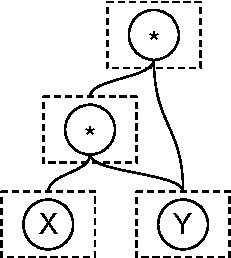
\includegraphics[scale=0.5]{XYY} \qquad 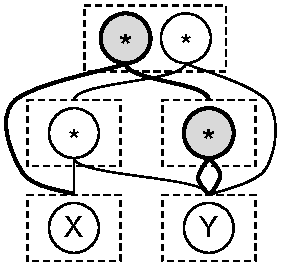
\includegraphics[scale=0.5]{assoc} \qquad 
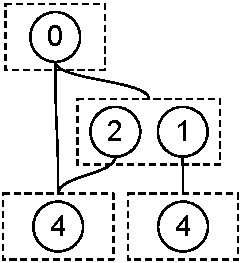
\includegraphics[scale=0.5]{CSE} 
    \vspace{7pt}
    \caption{Left: E-Graph representing $(X \times Y) \times Y$, and the graph after applying
      associativity to the root (middle). New nodes are in gray. Each dashed box is an E-Class.
      Right: the CSE problem. Each node shows its cost.}
    \label{assoc}
    \vspace{10pt}
\end{figure}

An E-Graph represents sets of equivalent expressions. A node in the graph is
called an E-Class, which contains the root operators of a set of equivalent
expressions. The edges are similar to the edges in an abstract syntax tree; but
instead of pointing from an operator directly to a child, each edge points from
an operator to an E-Class of expressions. For example, in Figure~\ref{assoc} the
top class in the middle represents the set of equivalent expressions \{$(X\times Y)\times Y,
X\times (Y\times Y)$\}. Note that the class represents two expressions, each with 2
appearances of $Y$ and one appearance of $X$, whereas each variable only appears
once in the E-Graph. This is because the E-Graph makes sure its expressions share
all possible common subexpressions. As the size of the graph grows, this
compression becomes more and more notable; in some cases a graph can 
represent a number of expressions exponential to its
size \cite{DBLP:journals/corr/abs-1012-1802}. We take advantage of this
compression in SPORES to efficiently cover vast portions of the search
space. If saturation, as described below, carries out to convergence, the E-Graph represents the search space exhaustively. 

An E-Graph can also be seen as an AND-OR DAG over expressions. Each E-Class is an OR node whose children are equivalent expressions from
which the optimizer chooses from. Each operator is an AND node whose children must all be picked if the operator itself is picked. In this dissertation we favor the terms E-Graph and E-Class to emphasize each OR node is an equivalence class. 

\subsubsection*{Saturating the E-Graph}
At the beginning of the optimization process, the optimizer instantiates the
graph by inserting the nodes in the syntax tree of the input expression one by
one in post order. For example, for input $(X\times Y)\times Y$, we construct the left graph
in Figure~\ref{assoc} bottom-up. By inserting in post order, we readily exploit
existing common subexpressions in the input. Once the entire input expression is
inserted, the optimizer starts to extend the graph with new expressions equivalent to
the input. It considers a list of equations, and matches either side of the
equation to subgraphs of the E-Graph. If an equation matches, the optimizer then
inserts the expression on the other side of the equation to the graph. For
example, applying the associativity rule extends the left graph in
Figure~\ref{assoc} with $X\times (Y\times Y)$, resulting in the right graph.
Figure~\ref{eqsat} shows the pseudo code for this process. While inserting new
expressions, the optimizer checks if any subexpression of the new expression is
already in the graph. If so, it reuses the existing node, thereby exploiting all
possible common-subexpressions to keep the E-Graph compact. In
Figure~\ref{assoc}, only two $\times$ are added since the variables $X$ and $Y$ are
already in the graph. Once the entire new expression has been added, the
optimizer then merges the newly created E-Class at its root with the E-Class
containing the matched expression, asserting them equal. Importantly, the
optimizer also propagates the congruent closure of this new equality. For
example, when $A+A$ is merged with $2\times A$, the optimizer also merges $(A+A)^2$
with $(2\times A)^2$. Figure~\ref{eqsat} shows the pseudo code for adding an
expression to E-Graph. This process of match-and-insert is repeated until the
graph stops changing, or reaching a user-specified bound on the number of 
saturation iterations. If this process does converge, that means no rule can add new
expressions to the graph any more. If the set of rules are complete, as is our
$R_{EQ}$, convergence of saturation implies the resulting E-Graph represents
the transitive closure of the equality rules applied to the initial expression.
In other words, it contains \textit{all} expressions equivalent to the input under the equality rules.

\begin{figure}
\begin{lstlisting}[language=Python]
def saturate(egraph, equations):
  for eq in equations: 
    matches = egraph.match(eq.lhs)
    for eclass in matches: 
      ec = egraph.add(eq.rhs)
      egraph.merge(eclass, c)

def add(expr):
  ID = egraph.find(expr)
  if ID != NULL:
    return ID
  else:
    cids = expr.children.map(add)
    ID = egraph.insert(expr.op, cids)
    return ID
\end{lstlisting}
    \caption{Equality saturation pseudocode. 
      % \texttt{match} returns the IDs of the root class of any matching subgraph;
      % \texttt{merge} combines two E-Classes given their IDs; it also propagates
      % the congruent closure of the new equality.
      % Figure~\ref{fig:egraphadd} defines \texttt{add}.
}
    \label{eqsat}
    \vspace{7pt}
\end{figure}
% \begin{figure}
% \begin{lstlisting}[language=Python]
% def add(expr):
%   ID = egraph.find(expr)
%   if ID != NULL:
%     return ID
%   else:
%     cids = expr.children.map(add)
%     ID = egraph.insert(expr.op, cids)
%     return ID
% \end{lstlisting}
%     \caption{Pseudo code for adding an expression to the E-Graph. 
%      % \texttt{find}
%      %  looks for the given expression in the E-Graph, and returns its root ID if
%      %  it already exists, or \texttt{NULL} otherwise. \texttt{insert} adds the
%      %  given operator to the E-Graph, and points its children to E-Classes with the
%      %  given class IDs. 
% }
%     \label{fig:egraphadd}
% \end{figure}

The outer loop that matches equations to the graph can be implemented by a more
efficient algorithm like the Rete algorithm \cite{DBLP:journals/ai/Forgy82} when
the number of equations is large. However, we did not find matching to be
expensive and simply match by traversing the graph. Our implementation uses the
E-Graph data structure from the \texttt{egg}~\cite{willsey2020egg} library. 
\subsubsection*{Dealing with Expansive Rules}
While in theory equality saturation will converge with well-constructed rewrite
rules, in practice the E-Graph may explode for certain inputs under certain rules. For example, a long
chain of multiplication can be rewritten to an exponential number of
permutations under associativity and commutativity (AC rules). If we 
apply AC rules everywhere applicable in each iteration, the graph would soon use
up available memory. We call this application strategy the \emph{depth-first}
strategy because it eagerly applies expansive rules like AC. 
AC rules by themselves rarely affect performance \rvb{\cite{DBLP:conf/edbt/KernertKL15}}, and
SystemML also provides the fused \texttt{mmchain} operator that efficiently computes
multiplication chains, so permuting a chain is likely futile. In practice, AC
rules are useful because they can enable other rewrites. Suppose we have a rule
$R_{factor}: A\times X + B\times X \rightarrow (A+B)\times X$ and an expression $U\times Y + Y\times V$.
Applying commutativity to $Y\times V$ would then transform the expression to be
eligible for $R_{factor}$. With this insight, we change each saturation
iteration to sample a limited number of matches to apply per rule, instead of
applying all matches. This amounts to adding \texttt{matches = sample(matches, limit)} between line 3 and line 4 in Figure~\ref{eqsat}. 
Sampling encourages each rule to be considered equally often
and prevents any single rule from exploding the graph. This helps ensure good
exploration of the search space when exhaustive search is impractical. 
But when it is
possible for saturation to converge and be exhaustive, it still converges with high probability
when we sample matches. Our experiments in Section~\ref{overhead} show sampling
always preserve convergence in practice.

\subsubsection*{Extracting the Optimal Plan}
\label{extraction}

A greedy strategy to extract the best plan from the saturated E-Graph is to
traverse the graph bottom-up, picking the best plan at each level. This assumes
the best plan for any expression also contains the best plan for any of its
subexpressions. However, the presence of common subexpressions breaks this
assumption. In the right-most graph in Figure~\ref{assoc} each operator 
node is annotated with its cost. 
Between the nodes with costs 1 and 2, a greedy strategy would choose 1, which
incurs total cost of $1+4=5$. The greedy strategy then needs to pick the root
node with cost 0 and the other node with cost 4, incurring a total cost of 9. 
However, the optimal strategy is to pick the nodes with 0, 2 and share the same
node with cost 4, incurring a total cost of 6. 

We handle the complexity of the search problem with a constraint
solver. We assign a variable to each operator and each E-Class, then construct
constraints over the variables for the solver to select operators that make up a
valid expression. The solver will then optimize a cost function defined over the
variables; the solution then corresponds to the optimal expression equivalent to
the input. \rvo{We implement both the greedy strategy and the solver-based strategy and compare them
in Section~\ref{overhead}.} 

\subsubsection*{Constraint Solving and Cost Function}
We encode the problem of extracting the cheapest plan from the E-Graph with
integer linear programming (ILP). Figure~\ref{ilp} shows this encoding. For each
operator in the graph, we generate a boolean variable $B_{op}$; for each E-Class
we generate a variable $B_c$. For the root class, we use the variable $B_r$.
Constraint $F(op)$ states that if the solver selects an operator, it must also
select all its children; constraint $G(c)$ states that if the solver selects an
E-Class, it must select at least one of its members. Finally, we assert $B_r$ must 
be selected, which constrains the extracted expression
to be in the same E-Class as the unoptimized expression. These three constraints together
ensure the
selected nodes form a valid expression equivalent to the unoptimized input.
Satisfying these constraints, the solver now minimizes the cost function given
by the total cost of the selected operators. Because each $B_{op}$ represents an
operator node in the E-Graph which can be shared by multiple parents, this
encoding only assigns the cost once for every shared common subexpression. In
our implementation, we use Gurobi~\cite{gurobi} to solve the ILP problem.

\begin{figure}
{\small
    \begin{align*}
Constraints &\equiv B_r \wedge \bigwedge_{op} F(op) \wedge \bigwedge_c G(c)
\\ F(op) &\equiv B_{op} \rightarrow \bigwedge_{c \in op.children} B_c \\ G(c)
&\equiv B_c \rightarrow \bigvee_{op \in c.nodes} B_{op}
\end{align*}
\[\textbf{minimize} \sum_{op} B_{op} \cdot C_{op} \textbf{ s.t. } Constraints\]
    \caption{ILP constraint and objective for extraction. }
    \vspace{-10pt}
    \label{ilp}
}%
\end{figure}
\begin{figure}
\begin{align*}
    \textbf{S}[X\times Y] &= min(\textbf{S}[X], \textbf{S}[Y]) \\ \textbf{S}[X+Y] &=
    min(1, \textbf{S}[X]+\textbf{S}[Y]) \\ \textbf{S}[\sum_i X] &= min(1, |i|
    \cdot \textbf{S}[X])
\end{align*}
    \caption[Sparsity estimation]{Sparsity estimation. We define $sparsity = nnz
      / size$, i.e. a 0 matrix has sparsity $0.0$\protect\footnotemark. $|i|$ is
      the size of the aggregated dimension. }
    \label{fig:cost}
\end{figure}
\footnotetext{Some may find this definition counter-intuitive; we define it so
  to be consistent with SystemML.}

Each operation usually has cost proportional to the output size in terms of
memory allocation and computation. Since the size of a matrix is proportional to
its the number of non-zeroes (nnz), we use SystemML's estimate of nnz as the
cost for each operation. Under our relational interpretation, this corresponds
to the cardinality of relational queries. We use the simple estimation scheme in
Figure~\ref{fig:cost}, which we find to work well. \rvb{We rely on SystemML's 
estimation for non-sum-product operators.} Future work can hinge on the
vast literature on sparsity and cardinality estimation to improve the cost
model.

\subsection{Schema and Sparsity as Class Invariant}
In the rules $R_{EQ}$ used by the saturation process, Rule~(\ref{RRC_ma}) If $i
\not\in A$, $A \times \sum_i B = \sum_i (A \times B)$ contains a condition on attribute
$i$ which may be deeply nested in the expression. This means the optimizer
cannot find a match with a simple pattern match. Fortunately, all expressions in
the same class must contain the same set of free attributes (attributes not
bound by aggregates). In other words, the set of free variables is invariant
under equality. This corresponds precisely to the schema of a database -
equivalent queries must share the same schema. We therefore annotate each class
with its schema, and also enable each equation to match on the schema.

In general, we find class invariants to be a powerful construct for programming
with E-Graphs. For each class we track as class invariant if there is a constant
scalar in the class. As soon as all the children of an operator are found to
contain constants, we can fold the operator with the constant it computes. This
seamlessly integrates constant folding with the rest of the rewrites. We also
treat sparsity as a class invariant and track it throughout equality saturation.
Because our sparsity estimation is conservative, equal expressions that use
different operators may have different estimates. But as soon as we identify
them as equal, we can merge their sparsity estimates by picking the tighter one,
thereby improving our cost function. Finally, we also take advantage of the
schema invariant during constraint generation. Because we are only interested in
RA expressions that can be translated to LA, we only generate symbolic variables
for classes that have no more than two attributes in their schema. This prunes
away a large number of invalid candidates and helps the solver avoid wasting
time on them. We implement class invariants using \texttt{egg}'s Metadata API.

\subsection{Translation, Fusion and Custom Functions}
\label{udfs}
Since equality saturation can rewrite any expression given a set of equations,
we can directly perform the translation between LA and RA within saturation,
simply by adding the translation rules $R_{LR}$ from Figure~\ref{RMR}.
Furthermore, saturation has flexible support for custom functions. The simplest
option is to treat a custom functions as a black box, so saturation can still
optimize below and above them. With a little more effort, we have the option to
extend our equations $R_{EQ}$ to reason about custom functions, removing the
optimization barrier. We take this option for common operators that are not part
of the core RA semantics, e.g. square, minus and divide. In the best scenario,
if the custom function can be modeled by a combination of basic operators, we
can add a rule equating the two, and retain both versions in the same graph for
consideration. In fact, this last option enables us to encode fused operators
and seamlessly integrate fusion with other rewrite rules. As a result, the
compiler no longer need to struggle with ordering fusion and rewrites, because
saturation simultaneously considers all possible ordering. 
\rvo{We note that although supporting custom functions require additional rules in
\sys, these rules are all identities, and they are much simpler than the heuristics
rules in SystemML which need to specify when to fire a rule and how each rule
interacts with another.} \rvt{Finally, although 
SystemML does not directly expose ``physical'' operators, e.g. different matrix
multiplication algorithms, \sys\ readily supports optimization of physical plans. 
For example, we could use two distinct operators for two matrix multiplication 
algorithms, and both would always appear in the same E-Class. Both operators
would share the same child E-Classes, therefore the additional operator only
adds one node for every class that contains a matrix multiply.}

\subsection{Saturation v.s. Heuristics}

Using equality saturation, SPORES elegantly remedies the drawbacks of
heuristics mentioned in the beginning of section~\ref{explore}. First, when two
or more conflicting rewrites apply, they would be added to the same E-Class, and
the extraction step will pick the more effective one based on the global cost
estimate. Second, there is no need to carefully order rewrites, because
saturation simultaneously considers all possible orders. For example, when rules
$R_1$ and $R_2$ can rewrite expression $e$ to either $R_1(R_2(e))$ or
$R_2(R_1(e))$, one iteration of saturation would add $R_1(e)$ and $R_2(e)$ to
the graph, and another iteration would add both $R_1(R_2(e))$ and $R_2(R_1(e))$
to the same E-Class. Third, rules do not need to reason about their dependency on
input or program properties, because extraction uses a global cost model that
holistically incorporates factors like input sparsity and common subexpressions.
Finally, every rule application in saturation applies one step of rewrite on top
of those already applied, naturally composing complex rewrites out of simple
ones.

\subsection{Integration within SystemML}

We integrate SPORES into SystemML to leverage its compiler
infrastructure. \sys\ plugs into the algebraic rewrite pass in SystemML; it
takes in a DAG of linear algebra operations, and outputs the optimized DAG.
Within \sys, it first translates the LA DAG into relational algebra,
performs equality saturation, and finally translates the optimal expression back
into LA. We obtain matrix characteristics such as dimensions and sparsity
estimation from SystemML. Since we did not focus our efforts in supporting
various operators and data types unrelated to linear algebra computation (e.g.
string manipulation), we only invoke SPORES on important LA expressions
from the inner loops of the input program.

% \begin{figure}
%     \centering 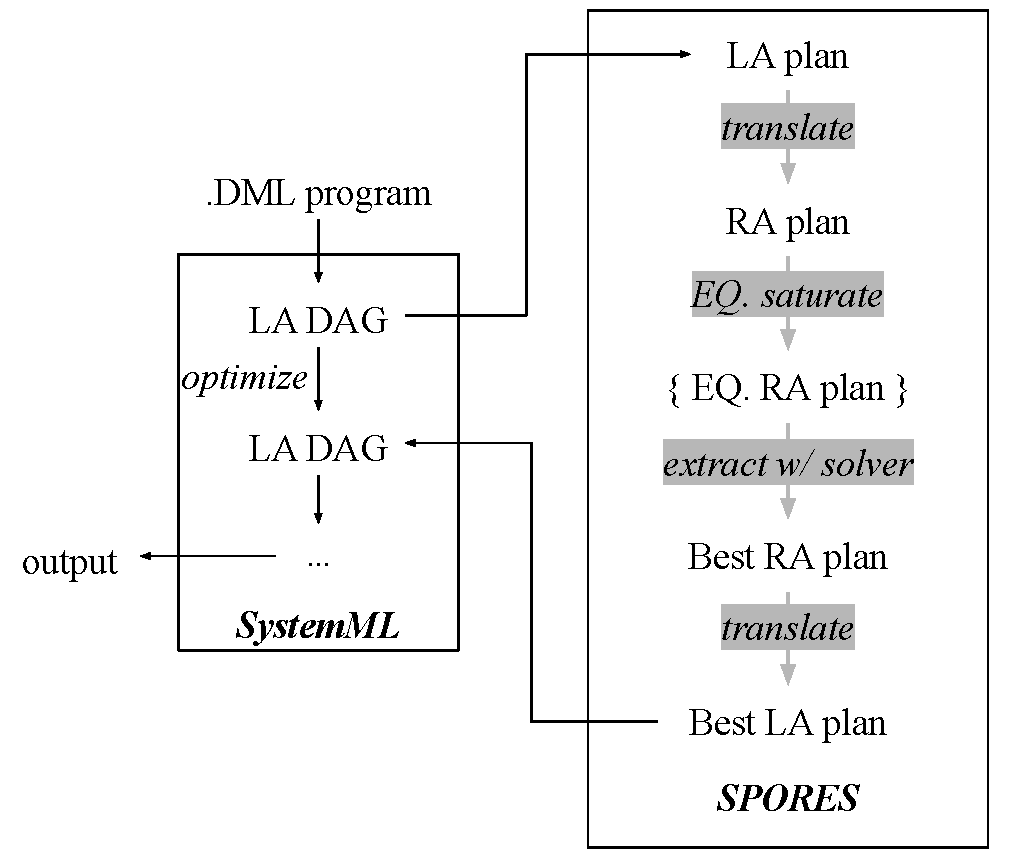
\includegraphics[width=0.6\linewidth]{arch}
%     \caption{Architecture of SPORES \& integration in SystemML}
%     \label{warp}
% \end{figure}{}

\section{Evaluation} \label{sec:evaluation}

We evaluate SPORES to answer three research questions about our
approach of relational equality saturation: 
\begin{itemize}
    \item \textbf{Section~\ref{relcomp}}: can SPORES derive hand-coded
      rewrite rules for sum-product optimization?
    \item \textbf{Section~\ref{perf}}: can SPORES find optimizations that
      lead to greater performance improvement than hand-coded rewrites and
      heuristics? 
      \item \textbf{Section~\ref{overhead}}: does SPORES induce compilation overhead afforded by its performance gain?  
\end{itemize}

We ran experiments on a single node with Intel E74890 v2 @ 2.80GHz with hyper-threading, 
1008 GB RAM, 1 Nvidia P100 GPU, 8TB
disk, and Ubuntu 16.04.6. We used OpenJDK 1.8.0, Apache Hadoop 2.7.3, and Apache
Spark 2.4.4. Spark was configured to run locally with 6 executors, 8
cores/executor, 50GB driver memory, and 100GB executor memory. Our baselines are
from Apache SystemML 1.2.0 and TensorFlow r2.1. We compile all TensorFlow functions
with XLA through \verb|tf.function|, and enable GPU.  

\subsection{Completeness of Relational Rules} \label{relcomp}
% \begin{figure}
% \begin{enumerate}
%   \item $sum(A+B) = sum(A)+sum(B)$
%   \item $sum(X^T) = sum(X)$
%   \item $sum(sum_{row}(X)) = sum(X)$,  $sum_{col}$ similar
%   \item $(UV)^T = V^TU^T$, $(U*V)^T=U^T*V^T$
%   \item $(A+B)^T=A^T + B^T$, $(X^T)^T=X$
%   \item $(X*Y)*Z = X*(Y*Z)$, $X*Y = Y*X$
%   \item $A * X + b * X =  (A+b)*X$
%   \item $a * UV = (a*U) V$
% \end{enumerate}
% \caption{LA equality rules $R_{LA}$ for comparison. \textcolor{red}{TODO fix caption}}
% \label{RLA}
% \end{figure}

% \begin{figure*}
%     \centering
%     \begin{tabular}{|l|c|l|}
%     \hline
%      Method Name & \# & Example Rewrite \\
%      \hline
     
% \verb|UnnecessaryOuterProduct| & 3 & \verb|X*(Y%*%1) ->| \verb| X*Y, if Y col vector |\\

% \verb|ColwiseAgg| & 3 & \verb|colsums(X) -> sum(X) or X, if col/row vector |\\

% \verb|RowwiseAgg| & 3 & \verb|rowsums(X) -> sum(X) or X, if row/col vector |\\

% \verb|ColSumsMVMult| & 1 & \verb|colSums(X*Y) -> t(Y) %*% X, if Y col vector |\\

% \verb|RowSumsMVMult| & 1 & \verb|rowSums(X*Y) -> X %*% t(Y), if Y row vector |\\

% \verb|UnnecessaryAggregate| & 9 & \verb|sum(X) -> as.scalar(X), if 1x1 dims |\\
% \verb|EmptyAgg| & 3 & \verb|sum(X) -> 0, if nnz(X)==0 |\\
% \verb|EmptyReorgOp| & 5 & \verb|t(X) -> matrix(0, ncol(X), nrow(X)) if nnz(X)==0|\\
% \verb|EmptyMMult| & 1 & \verb|X%*%Y -> matrix(0,...), if nnz(Y)==0|\\
% \verb|IdentityRepMatrixMult| & 1 & \verb|X%*%y -> X if y matrix(1,1,1) |\\
% \verb|ScalarMatrixMult| & 2 & \verb|X%*%y -> X*as.scalar(y), if y is a 1-1 matrix |\\
% \verb|pushdownSumOnAdd| & 2 & \verb|sum(A+B) -> sum(A)+sum(B) if dims(A)==dims(B) |\\

% \verb|DotProductSum| & 2 & \verb|sum(v^2) -> t(v)%*%v if ncol(v)==1 |\\
% \verb|reorderMinusMatrixMult| & 2 & \verb|(-t(X))%*%y -> -(t(X)%*%y) |\\

% \verb|SumMatrixMult| & 3 & \verb|sum(A%*%B) -> sum(t(colSums(A))*rowSums(B)) if not dot product|\\
% \verb|EmptyBinaryOperation| & 3 & \verb|X*Y -> matrix(0,nrow(X), ncol(X)) / X+Y->X / X-Y -> X |\\
% \verb|ScalarMVBinaryOperation| & 1 & \verb|X*y -> X*as.scalar(y), if y is a 1-1 matrix |\\
% \verb|UnnecessaryBinaryOperation| & 6 & \verb|X*1 -> X (dep: should come after rm unnecessary vectorize) |\\
% \verb|BinaryToUnaryOperation| & 3 & \verb|X*X -> X^2, X+X -> X*2, (X>0)-(X<0) -> sign(X) |\\
% \verb|MatrixMultScalarAdd| & 2 & \verb|eps+U%*%t(V) -> U%*%t(V)+eps, U%*%t(V)-eps -> U%*%t(V)+(-eps) |\\
% \verb|DistributiveBinaryOperation| & 4 & \verb|(X-Y*X) -> (1-Y)*X |\\
% \verb|BushyBinaryOperation| & 3 & \verb|(X*(Y*(Z%*%v))) -> (X*Y)*(Z%*%v) |\\
% \verb|UnaryAggReorgOperation| & 3 & \verb|sum(t(X)) -> sum(X) |\\
% \verb|UnnecessaryAggregates| & 8 & \verb|sum(rowSums(X)) -> sum(X) |\\
% \verb|BinaryMatrixScalarOperation| & 3 & \verb|as.scalar(X*s) -> as.scalar(X)*s |\\

% \verb|pushdownUnaryAggTransposeOperation| & 2 & \verb|colSums(t(X)) -> t(rowSums(X)) |\\
% \verb|pushdownCSETransposeScalarOperation| & 1 & \verb|a=t(X), b=t(X^2) -> a=t(X), b=t(X)^2 for CSE t(X) |\\

% \verb|pushdownSumBinaryMult| & 2 & \verb|sum(lamda*X) -> lamda*sum(X) if lamdba is scalar|\\
% \verb|UnnecessaryReorgOperation| & 2 & \verb|t(t(X))->X potentially introduced by other rewrites |\\
% \verb|TransposeAggBinBinaryChains| & 2 & \verb|t(t(A)%*%t(B)+C) -> B%*%A+t(C) |\\
% \verb|UnnecessaryMinus| & 1 & \verb|-(-X)->X potentially introduced by other rewrites |\\
% \hline
% \end{tabular}{}
%     \caption{Sum-product rewrites in SystemML. The first column lists the name for each rewrite method. Each 
%     method implements a number of rewrite patterns, and the second column shows how many. The last column shows an example rewrite for each method. Following SystemML's notation, scalars are in lower-case and matrices/vectors in upper-case. \texttt{\%*\%} is matrix multiply,  \texttt{t()} is transpose, and \texttt{nnz(X)} is the number of non-zeroes in $X$. 
%     Equality saturation derives rewrites form all 31 methods (84 patterns) with relational  rules. }
%     \label{rewritecomplete}
% \end{figure*}{}

Theoretically, our first hypothesis is validated by the fact that our relational
equality rules are complete w.r.t. linear algebra semantics. To test completeness in
practice\footnote{\textit{``I have only proved it correct, not tried it''} --
  Donald Knuth}, our first set of experiments check if SPORES
can derive the hand-coded sum product rewrite rules in SystemML. To do this, we
input the left hand side of each rule into SPORES, perform equality
saturation, then check if the rule's right hand side is present in the saturated
graph. The optimizer is able to derive
all 84 sum-product rewrite rules in SystemML using relational equality rules. 
Refer to the long version of this chapter \cite{SPORESarxiv} for a list of these rewrites. 
We believe replacing the 84 ad-hoc
rules with our translation rules $R_{LR}$ and equality rules $R_{EQ}$ would greatly
simplify SystemML's codebase. Together with equality saturation, our relational
rules can also lead to better performance, as we demonstrate in the next set of
 experiments.

% We then replace the RA equalities with the usual
% linear algebra equalities listed in Figure~\ref{RLA} and perform the same test.
% This time, the optimizer can only derive 33 out of 59 rules.
% TODO get number

% While we argue the experiment shows the benefit of RA rules over LA rules, one
% may wonder if we over-constrain the LA rules; perhaps 
% by adding a few additional rules, the LA rules can become complete as well. To
% this we answer that our RA rules can be viewed as an enhanced version of LA
% rules. While there may be other alternatives, we have shown our rules to be apt
% both in theory and in practice. From a different angle, the rules in
% Figure~\ref{rewritecomplete} from SystemML can also be regarded as an enhanced
% version of LA equalities. However, it is incomplete because it cannot derive 
% our example optimization of $sum((X-UV^T)^2)$. Practically, our RA rules are both more
% principled and simpler than the hand-coded rules, so adopting the former can
% simplify the codebase and alleviate maintenance burden. Together with equality saturation, our RA
% rules can also lead to better performance, as we demonstrate in the next set of
% experiments.

% TODO runtime evaluation 
\subsection{Run Time Measurement} \label{perf}
We compare SPORES against SystemML's native optimizations for their
performance impact. As baseline, we run SystemML with optimization level 2 (\texttt{opt2}),
which is its default and includes all advanced rewrites like constant folding
and common subexpression elimination. We additionally enable SystemML's native
sum-product rewrites and operator fusion. \rvo{When using SPORES, we disable SystemML's
native sum-product rewrites, which means disabling the 84 rules discussed in Section~\ref{relcomp}.
We compile and execute 5 real-world
algorithms including Generalized Linear Model (GLM), Multinomial
 Logistic Regression (MLR), Support Vector Machine (SVM), Poisson
 Nonnegative Matrix Factorization (PNMF), and Alternating Least Square
 Factorization (ALS). We configure GLM and MLR to learn a probit model as a binary classifier.
 We take the implementation of these algorithms from
 SystemML's performance benchmark suite \cite{smlperftest}. All algorithms were used as benchmarks in previous
 optimization research \cite{ElgamalLBETRS17} \cite{DBLP:journals/pvldb/BoehmRHSEP18}.
We use the same input datasets from
\cite{DBLP:journals/pvldb/BoehmRHSEP18}, specifically the Amazon books review dataset
(Amazon/A) \cite{DBLP:conf/www/HeM16}, the Airline on-time performance dataset (Flights/F) \cite{flights},
the Netflix movie rating dataset (Netflix/N) \cite{netflix}, and the MNIST8M dataset (MNIST/M) \cite{mnist}.
In order to fit the computation in memory, we down sample each dataset to obtain inputs of small, medium and large sizes.
For the Amazon and Netflix data, AS/NS contian 25k reviews, AM/NM 50k, and AL/NL 100k. We convert the data
to a review matrix, where columns are items and rows are customers, then use it as input to ALS and PNMF. 
For the Flights and MNIST
datasets, FS/MS contain 2.5M rows, FM/MM 5M, and FL/ML 10M. We use these datasets as input to GLM / MLR / SVM.
Each algorithm learns if a flight is delayed more than 5 hours, or if an image shows the digit 2. In TensorFlow experiments we generate random inputs
that match the size of the intermediate data in the corresponding benchmark.}  
\rvt{
Our approach focuses on optimizing sum-product operations with the assumption that these operations take up the
majority of run time in machine learning programs. We test this assumption by profiling our benchmark programs
on the largest version of each dataset. Figure~\ref{heavy} shows that for each program on each input dataset,
sum-product operations including matrix multiply, addition, point-wise multiply and summation together take up
the great majority of run time (from 77.4\% to 98.9\%). For other heavy-hitting operations, we implement
standard rewrite rules as discussed in Section~\ref{udfs}.} 
\begin{figure}
    \centering  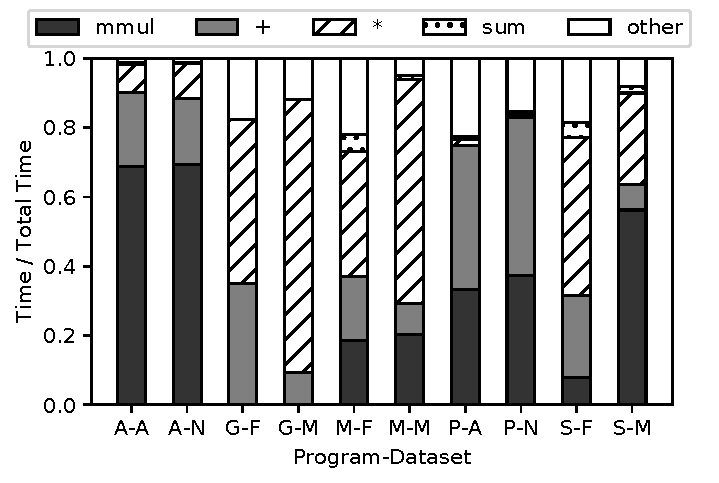
\includegraphics[width=0.8\linewidth]{heavy.pdf}
    \caption{\rvt{Run-time profile of benchmark programs.}}
    \label{heavy}
    \vspace*{5pt}
\end{figure}
Figure~\ref{eval} shows the program run time under \sys\ optimization against SystemML's
optimization. 
 \sys\ is competitive with the hand-coded rules
in SystemML: for GLM and SVM, \sys\ discovers the same
optimizations as SystemML does. For ALS, MLR and PNMF,
\sys\ found new optimizations that lead to \rvo{up to 10X speedup}.
We next analyze each benchmark in detail. 
\begin{figure}
    \centering  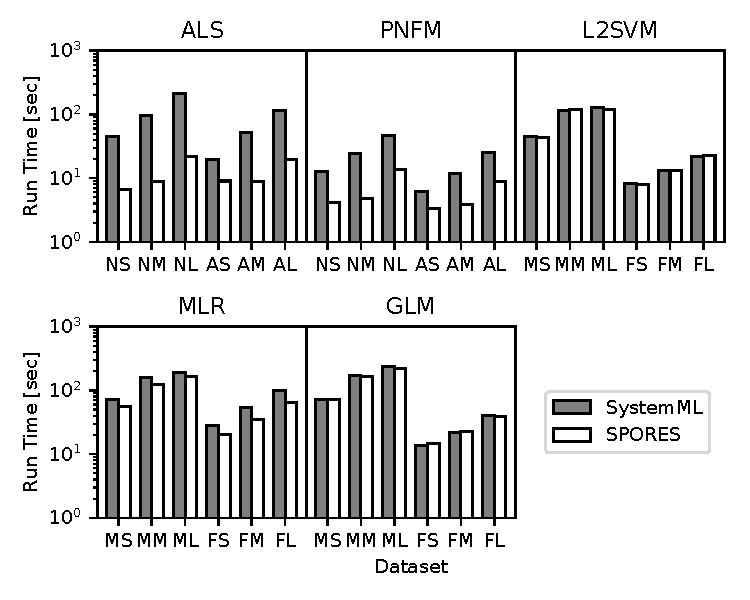
\includegraphics[width=0.9\linewidth]{runtime.pdf}
    \caption{\rvo{Run time under SystemML/SPORES compilation.}} 
    \label{eval}
    \vspace{5pt}
\end{figure}

% \begin{figure}[t]
% \begin{lstlisting}[language=R]
% H=H*(t(W)%*%(X/(W%*%H+eps)))/t(colSums(W))
% W=W*((X/(W%*%H+eps))%*%t(H))/t(rowSums(H))
% obj=sum(W%*%H)-sum(X*log(W%*%H+eps))
% \end{lstlisting}
%     \caption{PNMF main loop. $X$ is a sparse matrix, $W$ and $H$ are low-rank matrices, and
%       $eps$ is a scalar.}
%     \label{pnmf}
% \end{figure}
% \begin{figure}[t]
% \begin{lstlisting}[language=R]
% Q=P[,1:K] * (X %*% ssX_V)
% HV=t(X)%*%(Q - P[,1:K]
%       *(rowSums(Q)%*%matrix(1,1,K)))
% \end{lstlisting}
%     \caption{Part of MLogReg main loop. $X$ and $ssX\_V$ are matrices. In our experiment $K=1$ so
%       $P[,1:K]$ and $Q$ are column vectors, and $matrix(1,1,K)$ is a 1x1
%       matrix holding the value $1$. }
%     \label{mlogreg}
% \end{figure}



% TODO no section 
% \subsection{Rewrite Details} \label{optdetails}

For \textbf{ALS}, SPORES leads to up to 10X speedup beyond SystemML's
optimizations using our relational rules. Investigating the optimized code
reveals the speedup comes from a rather simple optimization: SPORES expands
$(UV^T - X)V$ to $UV^TV-XV$ to exploit the sparsity in $X$. Before the optimization,
all three operations (2 matrix multiply and 1 minus) 
in the expression create dense intermediates because $U$
and $V$ are dense. After the optimization, $XV$ can be computed efficiently thanks to
the sparsity in $X$. $UV^TV$ can be computed in one go without intermediates, taking advantage of
SystemML's \texttt{mmchain} operator for matrix multiply chains. Although the
optimization is straightforward, it is counter-intuitive because one expects
computing $A(B + C)$ is more efficient than $AB + AC$ if one does not consider
sparsity. For the same reason, SystemML simply does not consider distributing
the multiplication and misses the optimization.

For \textbf{PNMF}, the \rvo{speedup of up to 3.5X} using RA rules attributes to rewriting $sum(WH)$
to $sum_{col}(W) \cdot sum_{row}(H)$ which avoids materializing a dense
intermediate $WH$. Interestingly, SystemML includes this rewrite rule but did
not apply it during optimization. In fact, SystemML only applies the rule when
$WH$ does not appear elsewhere, in order to preserve common subexpression.
However, although $WH$ is shared by another expression in PNMF, the other
expression can also be optimized away by another rule. Because both rules uses heuristics to favor sharing CSE, neither fires. 
This precisely
demonstrates the limitation of heuristics. 

For \textbf{MLR}, \sys\ leads to \rvo{up to 1.3X speedup}. The important optimization\footnote{Simplified here for
  presentation. In the source code $P$ and $X$ are not variables but consist of
  subexpressions. } is $P * X - P * sum_{row}(P) * X$ to
$P*(1-P)*X$, where $P$ is a column vector. This takes advantage of the
\texttt{sprop} fused operator in SystemML to compute $P*(1-P)$, therefore
allocating only one intermediate. Note that the optimization factors out $P$, which
is the exact opposite to the optimization in ALS that distributes multiply. Naive
rewrite rules would have to choose between the two directions, or resort to
heuristics to break ties. 

% TODO check dimensions
% \begin{figure}[t]
% \begin{lstlisting}[language=R]
% out=1-Y*(Xw+step_sz*Xd);
% sv=(out>0);
% out=out*sv;
% g=wd+step_sz*dd-sum(out*Y*Xd); 
% h=dd+sum(Xd*sv*Xd);
% step_sz = step_sz - g/h;
% \end{lstlisting}
%     \caption{Part of L2SVM main loop. }
%     \label{l2svm}
% \end{figure}
% \begin{figure}[t]
% \begin{lstlisting}[language=R]
% t_gp=1.0/(1.0+abs(flt)*0.231641888)
% pt_gp = t_gp * ( 0.254829592 
%       + t_gp * (-0.284496736 
%       + t_gp * ( 1.421413741 
%       + t_gp * (-1.453152027 
%       + t_gp *   1.061405429))));
% \end{lstlisting}
%     \caption[gauss error function]{
%     Part of GLM main loop (approximates the Gauss error function~\cite{abramowitz+stegun}). $t\_gp$ is a matrix.}
%     \label{glm}
% \end{figure}
\rvb{
In summary, \sys\ improves performance consistently for ALS, PNMF and MLR across
different data sizes. The impact of sparsity on performance can be gleaned from the particular optimizations: ALS optimization takes advantage of sparsity, while PNMF and MLR optimizations apply for either dense or sparse inputs. }

For \textbf{SVM} and \textbf{GLM}, equality saturation finds the same optimizations as
SystemML does, leading to speedup mainly due to operator fusion. Upon
inspection, we could not identify better optimizations for \textbf{SVM}. For
\textbf{GLM}, however, we discovered a manual optimization that should improve
performance in theory, but did not have an effect in practice since SystemML
cannot accurately estimate sparsity to inform execution. 

\begin{figure}
    \centering  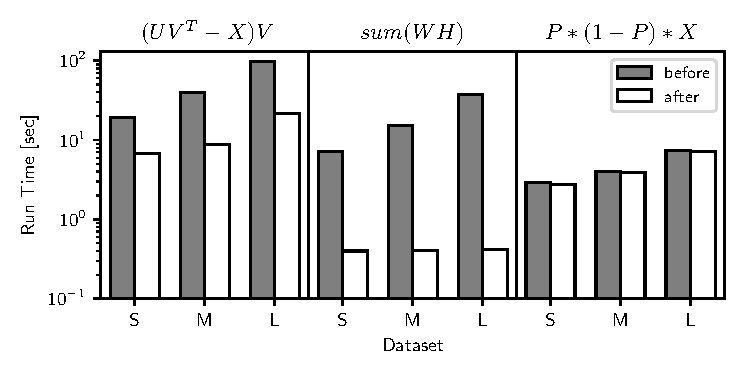
\includegraphics[width=0.9\linewidth]{tf.pdf}
    \caption{\rvb{Run time before- and after-rewrite in TensorFlow.}}
    \label{tfeval}
    \vspace{-10pt}
\end{figure}

\subsubsection*{Comparison Against TensorFlow}
\rvb{
We ran additional experiments in TensorFlow to see if it can also benefit from \sys's
optimizations. For each of the 3 rewrites we discussed in Section~\ref{perf}, we coded
the expressions before- and after-rewrite in TensorFlow. Then we compile each version
with TensorFlow XLA and measure its run time. Figure~\ref{tfeval} shows up to 90X and
50X speedup from the rewrites taken from ALS ($(UV^T-X)V$) and PNMF ($sum(WH)$) respectively. Upon inspection of
the compiled code, we found XLA performs no optimization on the input expressions, likely due
to certain heuristics preferring the unoptimized versions. For MLR ($P*(1-P)*X$),
XLA compiles the before- and after-rewrite expressions to the same code, so the run time
stays the same. We were unable
to compile our full benchmarks with XLA because the latter cannot compile certain operations
on sparse matrices. When this improves, we expect to see \sys\ bring its full potential
to TensorFlow. 
}
\subsection{Compilation Overhead} \label{overhead}
\begin{figure}
    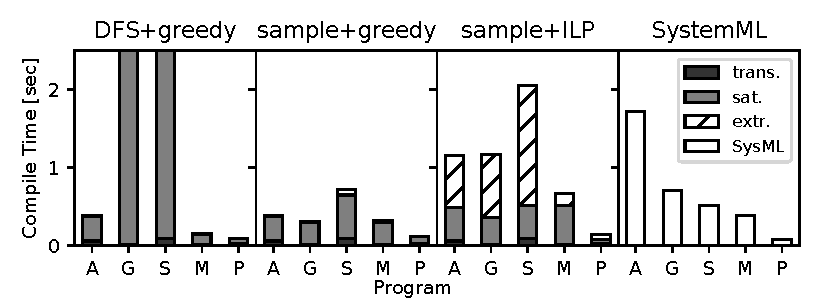
\includegraphics[width=\linewidth]{compiletime.pdf}
    \caption{Compile time breakdown for different saturation and extraction
      strategies. Depth-first saturation reaches the 2.5s timeout compiling GLM and SVM. }
    \label{compile}
    \vspace{5pt}
\end{figure}{}
\begin{figure}
    \centering  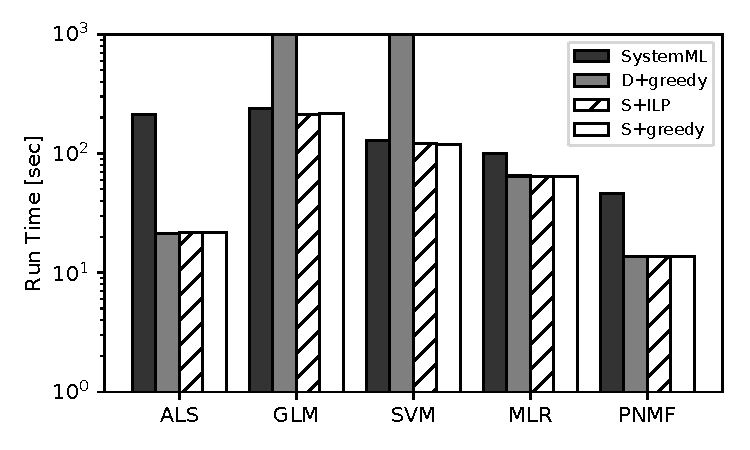
\includegraphics[width=0.8\linewidth]{strategy.pdf}
    \caption{\rvo{Performance impact of different saturation and extraction
      strategies. S is saturation with sampling, and D is depth-first saturation. Depth-first saturation runs into timeout compiling GLM and SVM.}} 
    \label{sampleeval}
\end{figure}

% TODO find number \textcolor{red}{TODO fix caption}}
In our initial experiments, SPORES induces nontrivial compilation
overhead compared to SystemML's native rule-based rewrites. Figure~\ref{compile}
 (sampling, ILP extraction) shows the compile time breakdown for each benchmark, and the majority of time is
spent in the ILP solver. We therefore experiment with the greedy algorithm 
described in Section~\ref{extraction}
 to see if we can trade off guarantees of optimality for a shorter
compile time. Figure~\ref{sampleeval}
shows the performance impact of greedy extraction, and Figure~\ref{compile} (sampling, greedy extraction)
shows the compile time with it. Greedy extraction significantly reduces compile
time without sacrificing \textit{any} performance gain! This is not surprising
in light of the optimizations we discussed in Section~\ref{perf}: all of
these optimizations improve performance regardless of common
subexpressions, so they are selected by both the ILP-based and the greedy
extractor.

We also compare saturation with sampling against depth-first saturation in terms of
performance impact and compile time. Recall the depth-first saturation strategy
applies all matches per rule per iteration. As Figure~\ref{compile} shows,
sampling is slightly slower for ALS, MLR and PNMF, but resolves the timeout for 
GLM and SVM. This is because sampling takes longer to converge when full
saturation is possible, and otherwise prevents the graph from blowing up before
reaching the iteration limit.
Indeed, saturation converges for ALS, MLR and PNMF, which means SPORES
can guarantee the optimality of its result under the given cost model. Saturation
does not not converge before reaching the iteration limit for GLM and SVM because
of deeply nested $*$ and $+$ in the programs. 
Convergence
may come as a surprise despite E-Graph's compaction -- expansive rules like
associativity and commutativity commonly apply in practice. However, the expression
DAGs we encounter are often small (no more than 15 operators), and large DAGs
are cut into small pieces by optimization barriers like uninterpreted functions. 

Figure~\ref{compile} compares the overall DAG compilation overhead of SystemML
against SPORES with different extraction strategies.
Note that the overhead of SystemML also includes optimizations unrelated to sum-product rewrites that are difficult to disentangle, therefore it only gives a sense of the base compilation time and does not serve as head-to-head comparison against SPORES. 
Although SPORES induces significant compilation overhead in light of the total DAG compilation time of SystemML, the overhead is afforded by
its performance gain. As we did not focus our efforts on
reducing compile time, we believe there is plenty room for improvement, for
example organizing rewrite rules to speed up saturation.

\subsection{Numerical Considerations} \label{evaldisc}
\rvt{
Although our rewrite rules preserve semantics for the reals, they do not
preserve semantics under floating point arithmetics. We therefore run experiments
to see if \sys\ sacrifices numerical accuracy. For L2SVM, we
compare the accuracy of the trained model under \sys\ / SystemML optimization; for
MLR and GLM we compare the $R^2$ value; PNMF and ALS terminate after some loss
falls below a threshold, therefore we compare the number of iterations until
termination. Table~\ref{tab:numeric} shows all these statistics are identical under
\sys\ / SystemML optimzation. Although \sys\ does not optimize for numerical accuracy,
equality saturation was used by Herbie \cite{DBLP:conf/pldi/PanchekhaSWT15} for that
exact purpose. We are actively collaborating with Herbie's authors to develop a
multi-objective optimizer for accuracy and run time. 
}
\begin{table}
    \centering
    \caption{\rvt{Numerical characteristics of compiled programs.}}
    \vspace*{7pt}
\scalebox{0.8}{
    \begin{tabular}{l|c|c|c|c}
    \hline
        Optimizer & SysML & SPORES & SysML & SPORES  \\
        \hline
        \hline
        Dataset & \multicolumn{2}{c|}{Airline} & \multicolumn{2}{c}{MNIST} \\
        \hline
        SVM ($acc.$) & $82.4\%$ & $82.4\%$ & $96.8\%$ & $96.8\%$ \\
        \hline
        MLR ($R^2$) & $0.773$ & $0.773$ & $0.742$ & $0.742$ \\
        \hline
        GLM ($R^2$) & 0.618 & 0.618 & 0.671 & 0.671 \\
        \hline
        \hline
        Dataset & \multicolumn{2}{c|}{Netflix} & \multicolumn{2}{c}{Amazon} \\
        \hline
        PNMF ($iter.$) & 18 & 18 & 36 & 36 \\
        \hline
        ALS ($iter.$) & 8 & 8 & 9 & 9 \\
        \hline
    \end{tabular}}
    \label{tab:numeric}
    \vspace*{5pt}
\end{table}{}

\section{Related Work}

% TODO emphasize SystemML
% TODO ADD Immanual Trummer, PILP
% Morpheus
% lara
% volcano
There is a vast body of literature for both relational query optimization and
optimizing compilers for machine learning. Since we optimize machine learning programs through a
relational lens, our work relates to research in both fields. As we have pointed
out, numerous state-of-the-art optimizing compilers for machine learning
 resort to syntactic rewrites and heuristics to optimize linear algebra
expressions~\cite{DBLP:reference/bdt/Boehm19}~\cite{DBLP:conf/icml/SujeethLBRCWAOO11}~\cite{DBLP:conf/sigmod/HuangB013}. We distinguish our work which performs optimization based on a
relational semantics of linear algebra and holistically explore the complex
search space. A majority of relational query optimization focus on join order
optimization \cite{Graefe95a} \cite{MoerkotteN06} \cite{MoerkotteN08}
\cite{selinger1979access}; we distinguish our work which optimizes programs with
join (product), union (addition), and aggregate (sum) operations. Sum-product optimization considers operators other than join while optimizing
relational queries. Recent years have seen a line of excellent theoretical and
practical research in this area \cite{KhamisNR16} \cite{Joglekar2016AJARAA}.
These work gives significant improvement for queries involving $\times$ and $\sum$,
but fall short of LA workloads that occur in practice. We step past these
frameworks by incorporating common subexpressions and incorporating addition
($+$). 

In terms of approach, our design of relational IR ties in to research that
explores the connection between linear algebra and relational algebra. Our
design and implementation of the optimizer ties into research that leverage
equality saturation and \textsc{and-or dag}s for query optimization and compiler
optimization for programming languages. Since we focus on optimizing sum-product
expressions in linear algebra, our work naturally relates to research in sum-product
optimization. We now discuss these three lines of research in detail. 

\subsection{Relational Algebra and Linear Algebra}
Elgamal et al. \cite{ElgamalLBETRS17} envisions \textsc{spoof}, a compiler for machine learning programs
that leverages relational query optimization techniques for LA sum-product optimization. 
We realize this vision by providing the translation
rules from LA to RA and the relational equality rules that completely represents
the search space for sum-product expressions. One important distinction is, Elgamal
et al. proposes \emph{restricted relational algebra} where every expression must
have at most two free attributes. This ensures every relational expression in every step of the
optimization process to be expressible in LA. In contrast, we remove this restriction and only require the 
optimized output to be in linear algebra. This allows us to trek out to spaces not
covered by linear algebra equality rules and achieve completeness. In addition 
to sum-product expressions, Elgamal et al. also considers selection and projection operations
like selecting the positive entries of a matrix. We plan to explore supporting
selection and projection in the future. Elgamal et al. also proposes compile-time generation of
fused operators, which is implemented by Boehm et al.~\cite{DBLP:journals/pvldb/BoehmRHSEP18}.
SPORES readily takes advantage of existing fused operators, and we
plan to explore combining sum-product rewrite with fusion generation in the future. 

MorpheusFI by Li et al.~\cite{DBLP:conf/sigmod/LiC019} and LARA by Hutchison et al.~\cite{DBLP:journals/corr/HutchisonHS17} explore optimizations across the interface of machine learning and database systems. In particular, MorpheusFI speeds up machine learning algorithms over large joins by pushing computation into each joined table, thereby avoiding expensive
materialization. LARA implements linear algebra operations with relational operations and
shows competitive optimizations alongside popular data processing systems. 
Schleich et al.\cite{DBLP:conf/sigmod/SchleichOC16} and Khamis et al.\cite{DBLP:journals/corr/NgoNOS17} explore in-database learning, which aims to push entire
machine learning algorithms into the database system. 
We contribute in this space by showing that even without a relational engine, the
relational abstraction can still benefit machine learning tasks as a powerful
intermediate abstraction. \rvt{Kotlyar et.al. \cite{DBLP:conf/europar/KotlyarPS97}
explore compiling sparse linear algebra via
a relational abstraction. We contribute by providing a simple set of rewrite rules
and prove them complete.}

\subsection{Equality Saturation and AND-OR DAGs}
Equality saturation and \textsc{and-or dag}s have been applied to optimize
low-level assembly code~\cite{DBLP:conf/pldi/JoshiNR02}, Java programs \cite{DBLP:journals/corr/abs-1012-1802}, 
database queries \cite{Graefe95a}, floating point arithmetics \cite{DBLP:conf/pldi/PanchekhaSWT15}, and even computer-aided
design models \cite{DBLP:journals/corr/abs-1909-12252}. The design of our relational IR brings unique challenges
in adopting equality saturation. Compared to database query optimizers 
that focus on optimizing join orders, unions and aggregates play a central
role in our relational IR and are prevalent in real-world programs. As
a result, our
equality rules depend on the expression schema which is not immediately accessible
from the syntax. We propose class invariants as a solution to access schema
information, and show it to be a powerful construct that enables constant
folding and improves cost estimation. Compared to optimizers for low-level
assembly code or Java program, we commonly encounter linear algebra expressions
that trigger expansive rules and make saturation convergence impractical. 
We propose to sample rewrite matches in order to achieve good exploration
without full saturation. Equality saturation takes advantage of constraint solvers which have also been applied to program optimization and query
optimization. In particular, the use of solvers for satisfiability
modulo theories by \cite{DBLP:conf/asplos/Solar-LezamaTBSS06} has spawned a paradigm now known as \textit{program synthesis}. 
In query optimization research, 
\cite{DBLP:conf/sigmod/Trummer017} applies Mixed Integer Linear Programming for optimizing join ordering. 
Although constraint solvers offer pleasing guarantees of optimality, our
experiments show their overhead does not bring significant gains for optimizing
LA expressions. 

\subsection{Low-level Code Generation}
\rvt{
Novel machine learning compilers including TACO \cite{DBLP:journals/pacmpl/KjolstadKCLA17},
TVM \cite{DBLP:conf/nips/ChenZYJMCGK18}, TensorComprehension \cite{DBLP:journals/corr/abs-1802-04730} and
Tiramisu \cite{DBLP:conf/cgo/BaghdadiRRSAZSK19} generate efficient low-level code
for kernel operators. These kernels are small expressions that consist of a few
operators. For example the MATTRANSMUL kernel in TACO implements $\alpha A^T x + \beta z$.
The kernels are of interest because they commonly appear in machine learning programs,
and generating efficient low-level implementation for them can greatly impact performance. 
However, these compilers cannot perform algebraic rewrite on large programs as \sys\ does.
For example, TACO
supports only plus, multiply and aggregate, whereas \sys\ supports any custom functions
as discussed in Section~\ref{udfs}; Tiramisu requires tens of lines of code just to
specify matrix multiply which is a single operator in \sys. Furthermore, the basic polyhedral
model in Tiramisu and TensorComprehension does not support sparse matrices. Sparse extensions exist, but require the
user to make subtle tradeoffs between expressivity and performance \cite{DBLP:journals/pieee/StroutHO18}.
At a high level,
we view these kernel compilers as complementary to \sys. The former can provide efficient kernel
implementation just like the fused operators in SystemML, and we can easily include these
kernels in \sys\ for whole-program rewrite. The TASO compiler \cite{DBLP:conf/sosp/JiaPTWZA19}
combines kernel-level rewrite with whole-program rewrite, and is
also driven by a set of equality rules like \sys. However, it induces significant overhead --
generating operator graphs with just up to 4 operators takes 5 minutes, and while \cite{DBLP:conf/sosp/JiaPTWZA19}
does not include detailed time for compiling whole programs, it reports the compilation
finishes in ``less than ten minutes''. In contrast, \sys\ takes seconds instead of minutes
in compilation.} 

% \subsection{Exploiting Sparsity}
% A number of optimizing compilers for linear algebra programs support sparse
% matrix operators . SystemML \cite{boehm2014systemml} and Cumulon
% \cite{DBLP:conf/sigmod/HuangB013} includes a variety of hand-fused sparse operators.
% \cite{ElgamalLBETRS17} further automates the generation of fused operator
% implementation. However, all existing approach either work on a per-operator
% basis, or rely on hand-coded rules to rewrite expressions to fused operators.
% Using equality saturation, we can automatically discover opportunity for
% operator fusion based on a simple set of equality rules. And even with the
% absence of operator fusion, we can still take advantage of sparsity in our
% optimization.

% \subsection{Multi-query Optimization}
% The research in Multi-query Optimization aims to share common subqueries among
% multiple queries to speed up processing \cite{Kathuria017}. This is closely
% related to our problem of exploiting CSEs in linear algebra, although our focus
% is intra-query instead of inter-query. Moreover, the majority of multi-query
% optimizers focus on joins, whereas union and aggregate are essential for linear
% algebra programs. One lesson we can learn from the literature multi-query
% optimization is to perform equality saturation for multiple expressions in the
% same egraph, thereby enabling sharing across optimization sessions and reducing
% compilation time.

\section{Limitations and Future Work}
\rvt{
We intend \sys\ to be used to optimize machine learning programs that perform
linear algebra operations. As such, \sys\ is not a linear algebra solver, and 
operations like matrix inversion and calculating eigenvalues are out of scope.
\sys\ does not include a matrix decomposition operator, but the programmer
can implement decomposition algorithms like our ALS and PNMF benchmarks. 
The operations we support already cover a variety of algorithms as we show in
the evaluation. Similar scope is shared by existing research \cite{DBLP:journals/pvldb/BoehmRHSEP18}
\cite{ElgamalLBETRS17}
\cite{DBLP:journals/pacmpl/KjolstadKCLA17}. Although
\sys\ does not focus on deep learning, its design can be adapted to optimize
deep models. We are experimenting to incorporate the identity rules from TASO
into our framework. It would be challenging to extend the completeness theorem to
the complex operators used in deep learning, 
but we expect our extension of equality saturation can find high-impact optimizations
with short compile time. Finally, although our rewrite rules are complete, we had to
resort to rule sampling and greedy extraction to cut down the overhead. Future work can 
investigate more intelligent rule application and extraction strategies. For example,
the optimizer can learn which rules more likely lead to performance improvement and
prioritizes firing those rules. Another direction is to incorporate plus into
theoretical sum-product frameworks like FAQ \cite{KhamisNR16} and guarantee optimality. 
}
